% !TEX root = 12_02.tex
\documentclass{article}
\usepackage{graphicx}

% Include your macro file (assuming it's named macros.tex or similar)
\input{../ARTICULO-ORIGINAL/macros.def}  % or \input{path/to/your/macros/file}

% Additional packages needed
\usepackage{natbib}     % For \citet command
\usepackage{hyperref}   % For \Cref
\usepackage{cleveref}   % For \Cref to work properly
\usepackage{bm}         % For bold math (used in your macros)
\usepackage{xspace}     % For \xspace (used in your macros)

% Define the missing \ours command
\newcommand{\ours}{CRATE}  % Replace with your actual model name

% Define identity matrix
\newcommand{\vI}{I}

% Define SSA and MSSA operators
\newcommand{\SSA}{\texttt{SSA}}
\newcommand{\MSSA}{\texttt{MSSA}}



% Define colors for syntax highlighting
\definecolor{codegreen}{rgb}{0,0.6,0}
\definecolor{codegray}{rgb}{0.5,0.5,0.5}
\definecolor{codepurple}{rgb}{0.58,0,0.82}
\definecolor{backcolour}{rgb}{0.95,0.95,0.92}

% Python style for listings
\usepackage{listings}

\lstdefinestyle{pythonstyle}{
    language=Python,
    backgroundcolor=\color{backcolour},
    commentstyle=\color{codegreen},
    keywordstyle=\color{magenta},
    numberstyle=\tiny\color{codegray},
    stringstyle=\color{codepurple},
    basicstyle=\ttfamily\footnotesize,
    breakatwhitespace=false,
    breaklines=true,
    captionpos=b,
    keepspaces=true,
    numbers=left,
    numbersep=5pt,
    showspaces=false,
    showstringspaces=false,
    showtabs=false,
    tabsize=4
}

\lstset{style=pythonstyle}





\begin{document}

{\centering \textsf{TFG Pepe}\par}

\vspace{0.5in}

{\huge jueves 12 febrero 2026}

\vspace{0.5in}

Hola José!
Esta semana hice lo acordado con respecto al dataset online, incluyendo el aumento de datos en caché; continue ``refactorizando'' y organizandome el codigo para los experimentos, tanto que ya ni me hace falta el \texttt{git} o el \texttt{tmux} y adicionalmete hice pruebas con una nueva arquitectura.  \\
Sobre el dataset, no tuve mucho problema y realmente va bastante más rápido. Valió la pena la charla. \\
Sobre lo de refactorizar, ahora estoy muy cómodo y me supone poco esfuerzo hacer cualquier prueba. Igual es un poco innecesario pero como no se que pruebas vamos a querer y aun soy muy joven e ilusionado, pues simplemente me apetece dedicar mi tiempo en eso :) \\
Antes de profundizar en la nueva arquitectura te quiero enseñar la seccion del articulo donde hablan de la visualizacion.

\vspace{0.5in}

We recapitulate the method to visualize attention maps in \citet{abnar2020quantifying, caron2021emerging}, at first specializing their use to instances of the \ours{} model before generalizing to the ViT.
\noindent
For the $k^{\mathrm{th}}$ head at the $\ell^{\mathrm{th}}$ layer of \ours{}, we compute the \textit{self-attention matrix} $\bfA_{k}^{\ell}\in\bbR^{n}$ defined as follows:
\begin{equation}\label{eq:def_attention_map_crate}
   \bfA_{k}^{\ell}= \begin{bmatrix} A_{k, 1}^{\ell} \\ \vdots \\ A_{k, N}^{\ell} \end{bmatrix} \in \bbR^{N}, \quad \text{where} \quad A_{k, i}^{\ell} = \frac{\exp(\ip{\vU^{\ell*}_k\vz^{\ell}_{i}}{\vU^{\ell*}_k\vz^{\ell}_{\mathrm{cls}}})}{\sum_{j=1}^{N}\exp(\ip{\vU^{\ell*}_k\vz^{\ell}_{j}}{\vU^{\ell*}_k\vz^{\ell}_{\mathrm{cls}}})}.   
\end{equation}
We then reshape the attention matrix $\bfA_{k}^{\ell}$ into a ${\sqrt{n}\times\sqrt{n}}$ matrix and visualize the heatmap as shown in (Figura 20, que es lo que queremos tu y yo). 
For example, the $i^{\mathrm{th}}$ row and the $j^{\mathrm{th}}$ column element of the heatmap in (Figura 20, que es lo que queremos tu y yo) corresponds to the $m^{\mathrm{th}}$ component of $\bfA_{k}^{\ell}$ if $m=(i - 1)\cdot \sqrt{n} + j$. 
In (Figura 20, que es lo que queremos tu y yo), we select 4 attention heads of \ours{} and visualize the attention matrix $\bfA_{k}^{\ell}$ for each image. 

\vspace{0.5in}

O sea, no parece que esté invirtiendo la red. Leyendo eso tampoco tengo claro porque habría resolución más allá del token. Estoy confuso con esto. De todas formas aún no implementé ninguna versión. Lo dejo para la próxima semana, o igual podríamos volver a hablarlo. \\

\section{Arquitectura propuesta}

\textbf{¿Por qué?} \\

En el articulo aproxima una matriz de forma $(I - A)$ como $(I + A)$, lo cual corresponde con el primer orden de \texttt{https://en.wikipedia.org/wiki/Neumann\_series}, lo cierto es que no conocía esto previamente y por tanto lo mire y lo entendí. De forma natural me pregunté, ¿Por qué no usar más orden? Intenté responder con lo que diría Yi Ma:

\begin{itemize}
	\item Primeramente pensé que era mala idea porque sería mas caro. Pero realmente no lo es mucho más y si bien vale la pena pues el coste computacional no es motivo.
	\item Después pensé en la simpleza. Yi Ma parece defender que CRATE es una obra científica y no de ingeniería, por tanto parecería natural quedarse sólo con lo más fundamental y obviar los \epmh{bells and whistles} como dirías tú. Pero realmente lo más científico es aproximar bien.
	\item Finalmente (ahora) pienso que Yi Ma, llegó al Transformer no de casualidad si no que lo deseaba, quería justificar lo conocido. Este me parece el motivo por el que Yi Ma se quedó en el primer order de Neumann.
\end{itemize}

Ahora te voy a explicar exactamente de que estoy hablando y que arquitectura nueva se deriva.

\vspace{0.5in}
Primero te muestro lo original por referencia. Aqui esta la matriz a invertir

\begin{equation}
    \nabla R^c(\vZ \mid \vU_{[K]})
    = \beta\sum_{k=1}^K \vU_k(\vU_k\adj\vZ)\Big(I +
    \beta(\vU_k\adj\vZ)\adj(\vU_k\adj\vZ)\Big)^{-1}.
    \label{eq:rate-gradient}
\end{equation}

Aqui la aproximación

\begin{align}\label{eq:gd_rc_neumann}
    \nabla R^{c}(\vZ \mid \vU_{[K]}) 
    &\approx \beta \sum_{k = 1}^{K}\vU_{k}(\vU_{k}\adj\vZ)\big(\vI - \beta (\vU_{k}\adj\vZ)\adj(\vU_{k}\adj\vZ)\big) \\
    &{\color{revision}= \beta \left(\sum_{k = 1}^{K}\vU_{k}\vU_{k}\adj\right)\vZ -  \beta^2\sum_{k = 1}^{K} \vU_{k}(\vU_{k}\adj\vZ)(\vU_{k}\adj\vZ)\adj(\vU_{k}\adj\vZ)}.
\end{align}

Finalmente

{\color{revision}\begin{equation}
    \vZ^{\ell + 1/2} = (1 - \beta \kappa) \vZ^{\ell} + \beta\kappa \MSSA{\vZ^{\ell} \mid \vU_{[K]}^{\ell}} \approx \vZ^{\ell} - \kappa\nabla R^{c}(\vZ^{\ell} \mid \vU_{[K]}^{\ell}),  \label{eq:gd-mcr-parts} 
\end{equation}}

Puedes revisar las definiciones de \texttt{SSA} y \texttt{MSSA} aquí \texttt{https://arxiv.org/pdf/2311.13110}

Ahora con el segundo orden la inversa quedaría (si entras en la wikipedia, T sería $-\beta (\vU_{k}\adj\vZ)\adj(\vU_{k}\adj\vZ)$ ):

\begin{align}\label{eq:gd_rc_neumann}
    \nabla R^{c}(\vZ \mid \vU_{[K]}) 
    &\approx \beta \sum_{k = 1}^{K}\vU_{k}(\vU_{k}\adj\vZ)\big(\vI - \beta (\vU_{k}\adj\vZ)\adj(\vU_{k}\adj\vZ) + \beta^2 ((\vU_{k}\adj\vZ)\adj(\vU_{k}\adj\vZ))^2  \big) \\
    &{\color{revision}= \beta \left(\sum_{k = 1}^{K}\vU_{k}\vU_{k}\adj\right)\vZ -  \beta^2\sum_{k = 1}^{K} \vU_{k}(\vU_{k}\adj\vZ)(\vU_{k}\adj\vZ)\adj(\vU_{k}\adj\vZ)  +  \beta^3\sum_{k = 1}^{K} \vU_{k}(\vU_{k}\adj\vZ)((\vU_{k}\adj\vZ)\adj(\vU_{k}\adj\vZ))^2 }. \\
    &{\color{revision}= \beta \vZ -  \beta^2\sum_{k = 1}^{K} \vU_{k}(\vU_{k}\adj\vZ)(\vU_{k}\adj\vZ)\adj(\vU_{k}\adj\vZ)  +  \beta^3\sum_{k = 1}^{K} \vU_{k}(\vU_{k}\adj\vZ)((\vU_{k}\adj\vZ)\adj(\vU_{k}\adj\vZ))\adj  ((\vU_{k}\adj\vZ)\adj(\vU_{k}\adj\vZ)  ) }.
\end{align}

Tomándonos la licencia de que $A^2 = A^{t}A$ es decir asumimos simetria en $U^{t}Z$. Que el sumatorio de utu es I ya lo dice el, pero lo pongo explitamente por espacio.

El tema esque ahora tenemos una atencion más. con signo opuesto


\begin{figure}[H]
\caption{a) es lo original b) lo que propongo}
\centering

\includegraphics[width=\linewidth]{figs/diagrama_red.drawio.png}
\end{figure}

\section{experimentos}

bueno pues lo implemente

hice experimentos con configuraciones identicas de mi red y la original.

\begin{lstlisting}[caption=la atencion, que es lo unico que cambia]
class Attention(nn.Module):
    def __init__(self, dim, heads=8, dim_head=64, dropout=0., order='first'):
        super().__init__()
        inner_dim = dim_head * heads
        project_out = not (heads == 1 and dim_head == dim)

        self.heads = heads
        self.scale = dim_head ** -0.5
        self.order = order  # 'first' or 'second'

        self.attend = nn.Softmax(dim=-1)
        self.dropout = nn.Dropout(dropout)

        self.qkv = nn.Linear(dim, inner_dim, bias=False)

        self.to_out = nn.Sequential(
            nn.Linear(inner_dim, dim),
            nn.Dropout(dropout)
        ) if project_out else nn.Identity()

    def forward(self, x):
        w = rearrange(self.qkv(x), 'b n (h d) -> b h n d', h=self.heads)

        # Compute (U^T Z)^T (U^T Z)
        dots = torch.matmul(w, w.transpose(-1, -2)) * self.scale

        if self.order == 'first':
            # First-order Neumann approximation
            # out = (U^T Z) * softmax((U^T Z)^T (U^T Z))
            attn = self.attend(dots)
            attn = self.dropout(attn)
            out = torch.matmul(attn, w)
        
        elif self.order == 'second':
            # Second-order Neumann approximation
            # out = out_1st - out_2nd
            
            # First order term: (U^T Z) * softmax((U^T Z)^T (U^T Z))
            attn_1st = self.attend(dots)
            attn_1st = self.dropout(attn_1st)
            out_1st = torch.matmul(attn_1st, w)
            
            # Second order term: (U^T Z) * softmax(((U^T Z)^T (U^T Z))^2)
            # Compute ((U^T Z)^T (U^T Z))^2
            dots_2nd = torch.matmul(dots, dots)
            attn_2nd = self.attend(dots_2nd)
            attn_2nd = self.dropout(attn_2nd)
            out_2nd = torch.matmul(attn_2nd, w)
            
            # Combine: subtract second order correction
            out = out_1st - out_2nd
        
        else:
            raise ValueError(f"order must be 'first' or 'second', got {self.order}")

        out = rearrange(out, 'b h n d -> b n (h d)')
        return self.to_out(out)

\end{lstlisting}

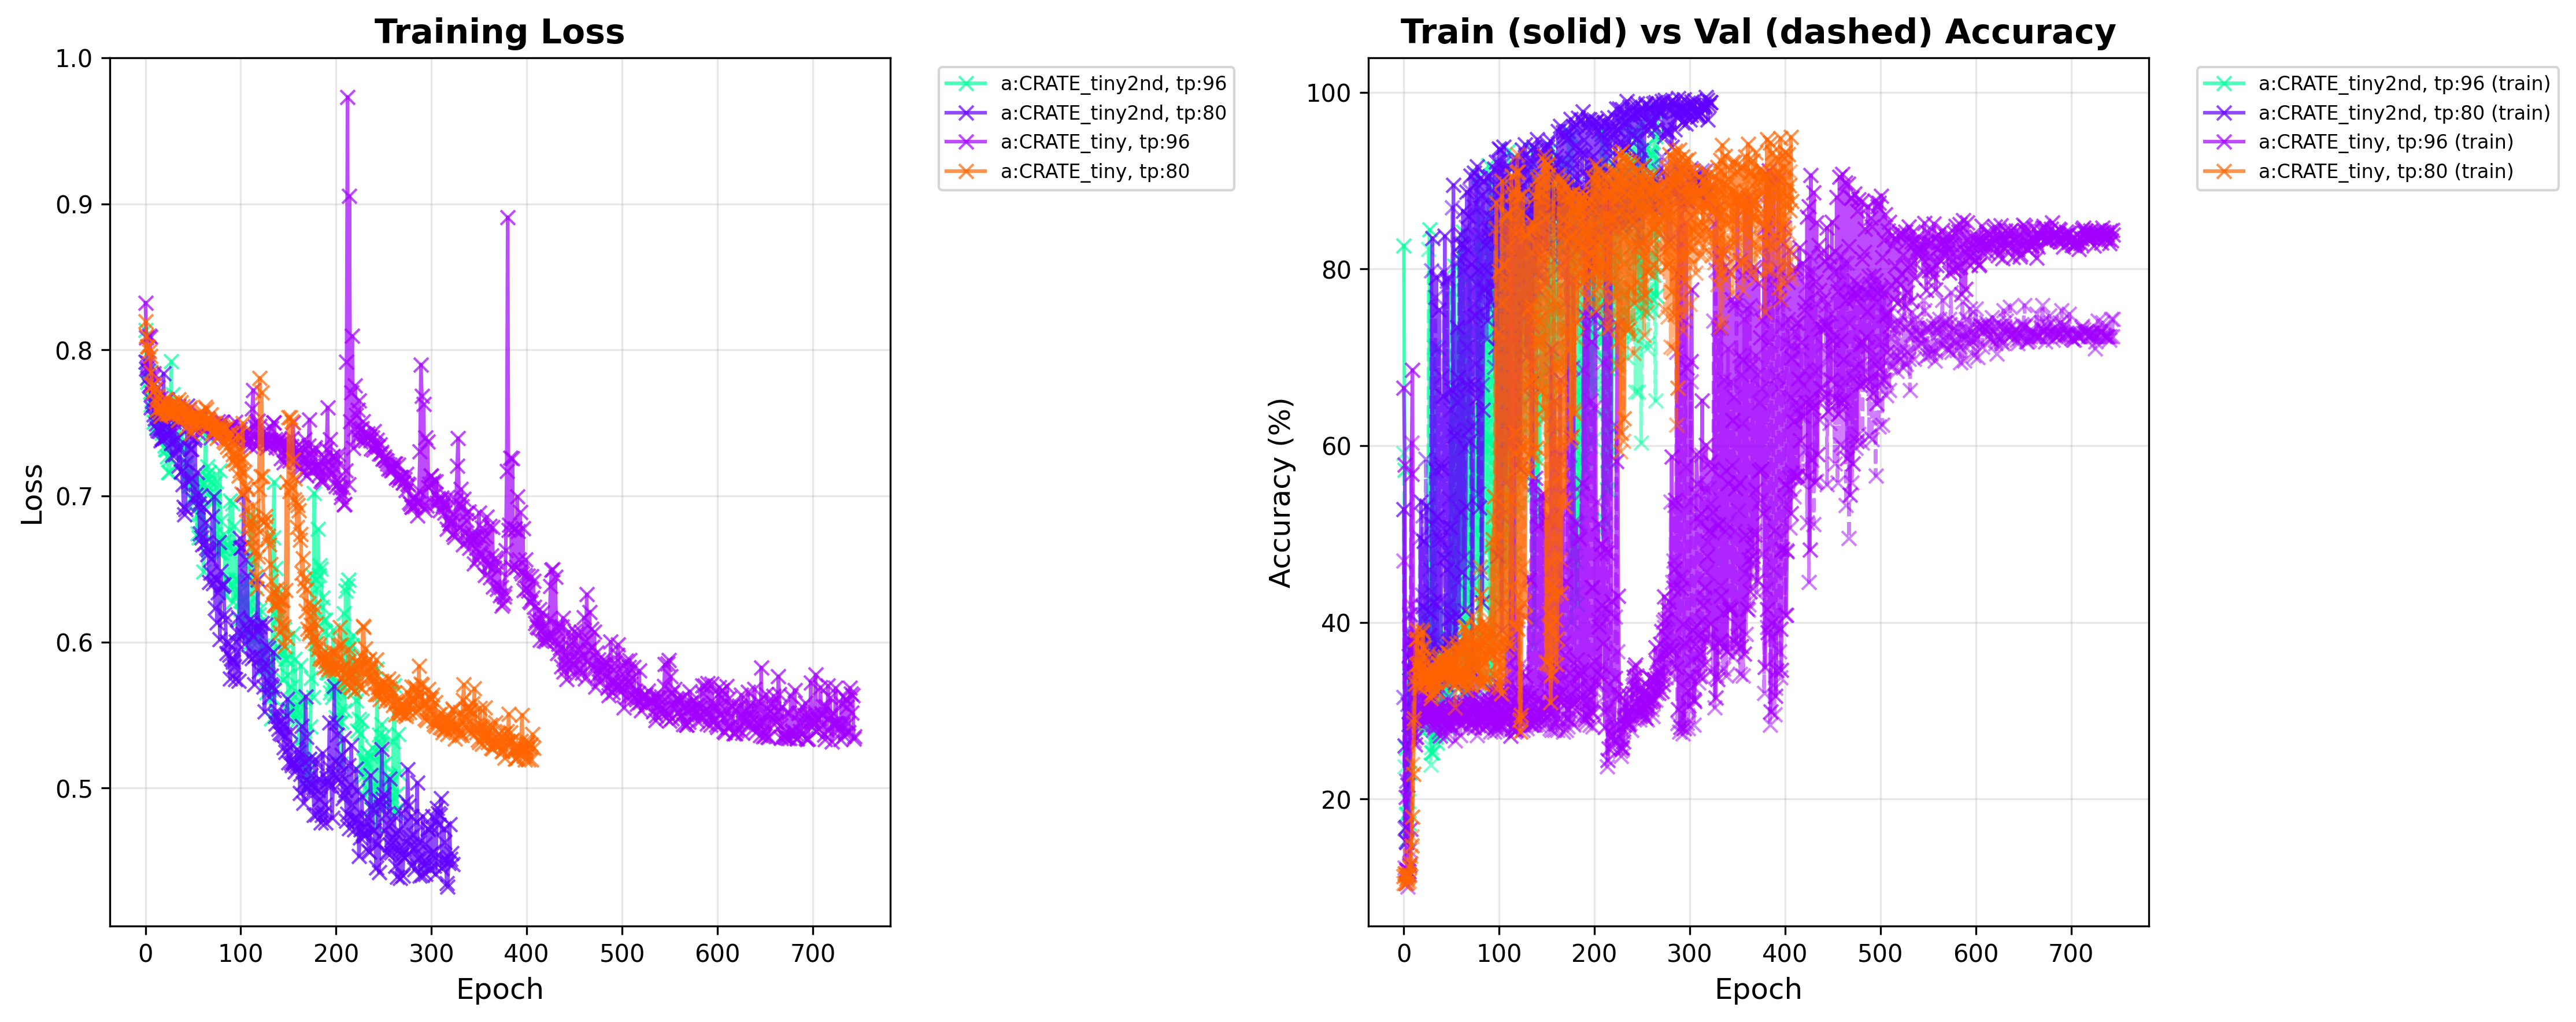
\includegraphics[width=\linewidth]{figs/9f3e62_e9f202_29b200_7bb28b_.png}


\begin{figure}[H]
	\caption{sparsidad de mi red}
\centering
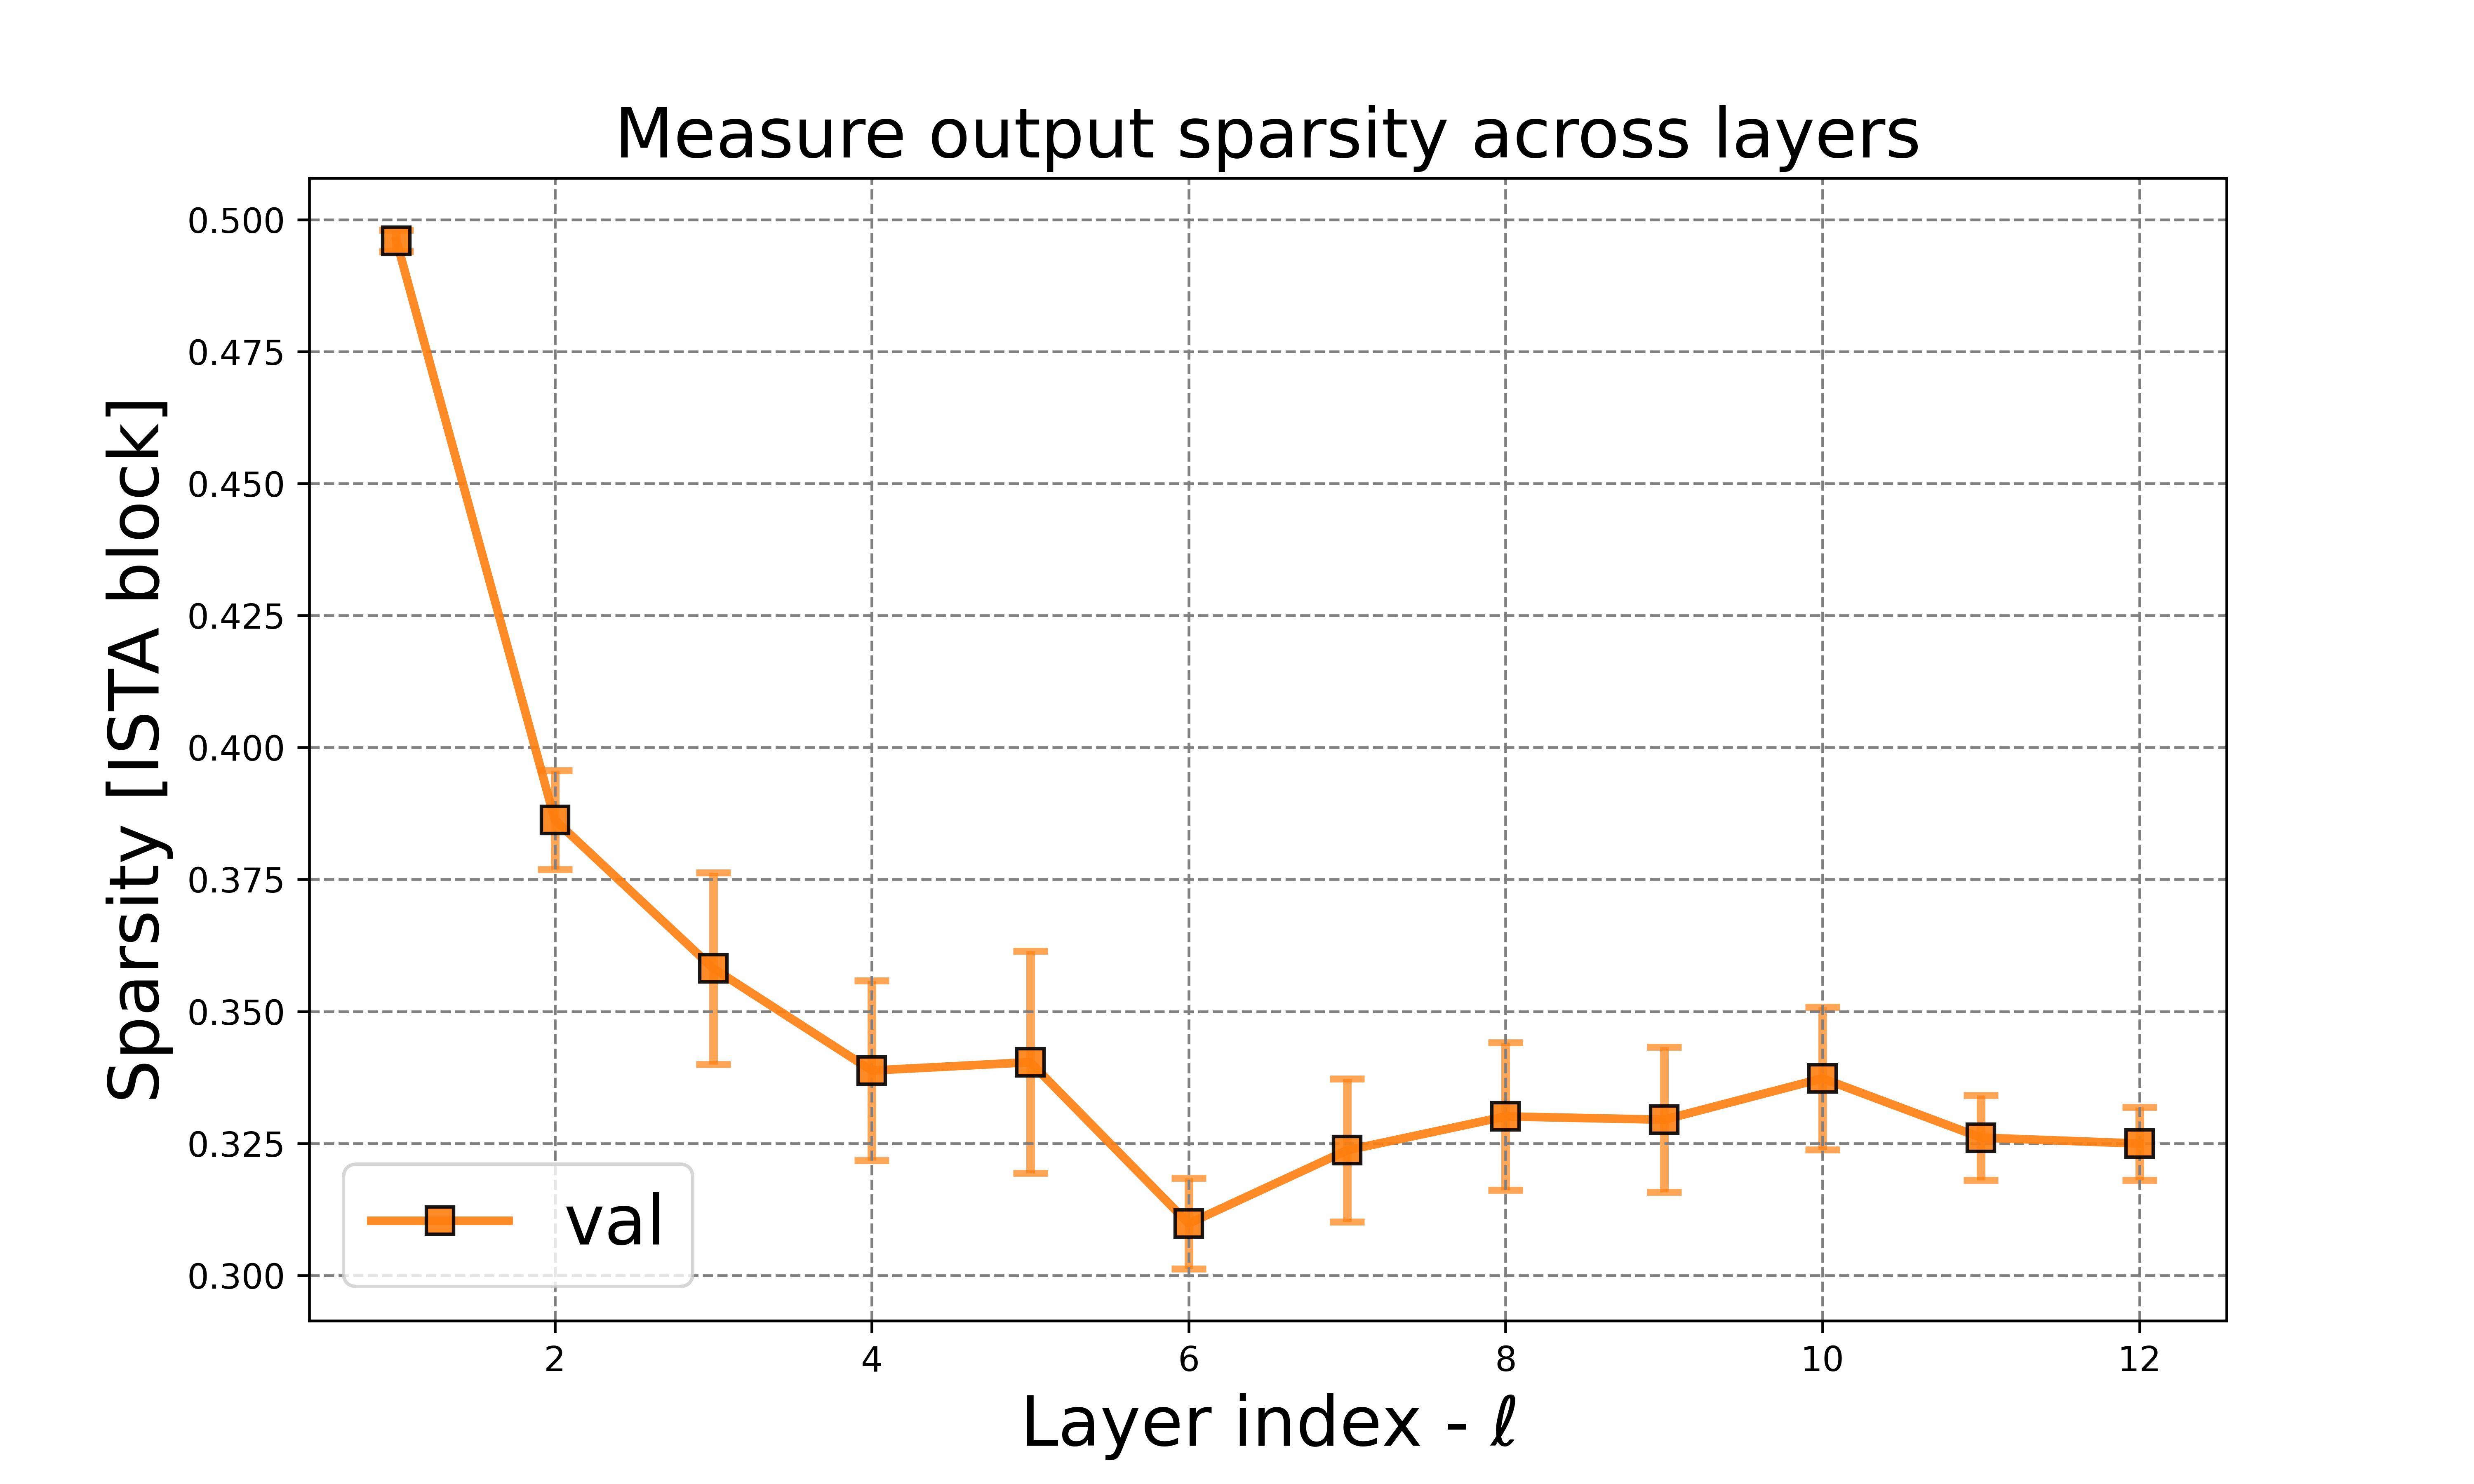
\includegraphics[width=\linewidth]{figs/mio_sparsity.png}
\end{figure}



\begin{figure}[H]
	\caption{sparsidad de su red}
\centering
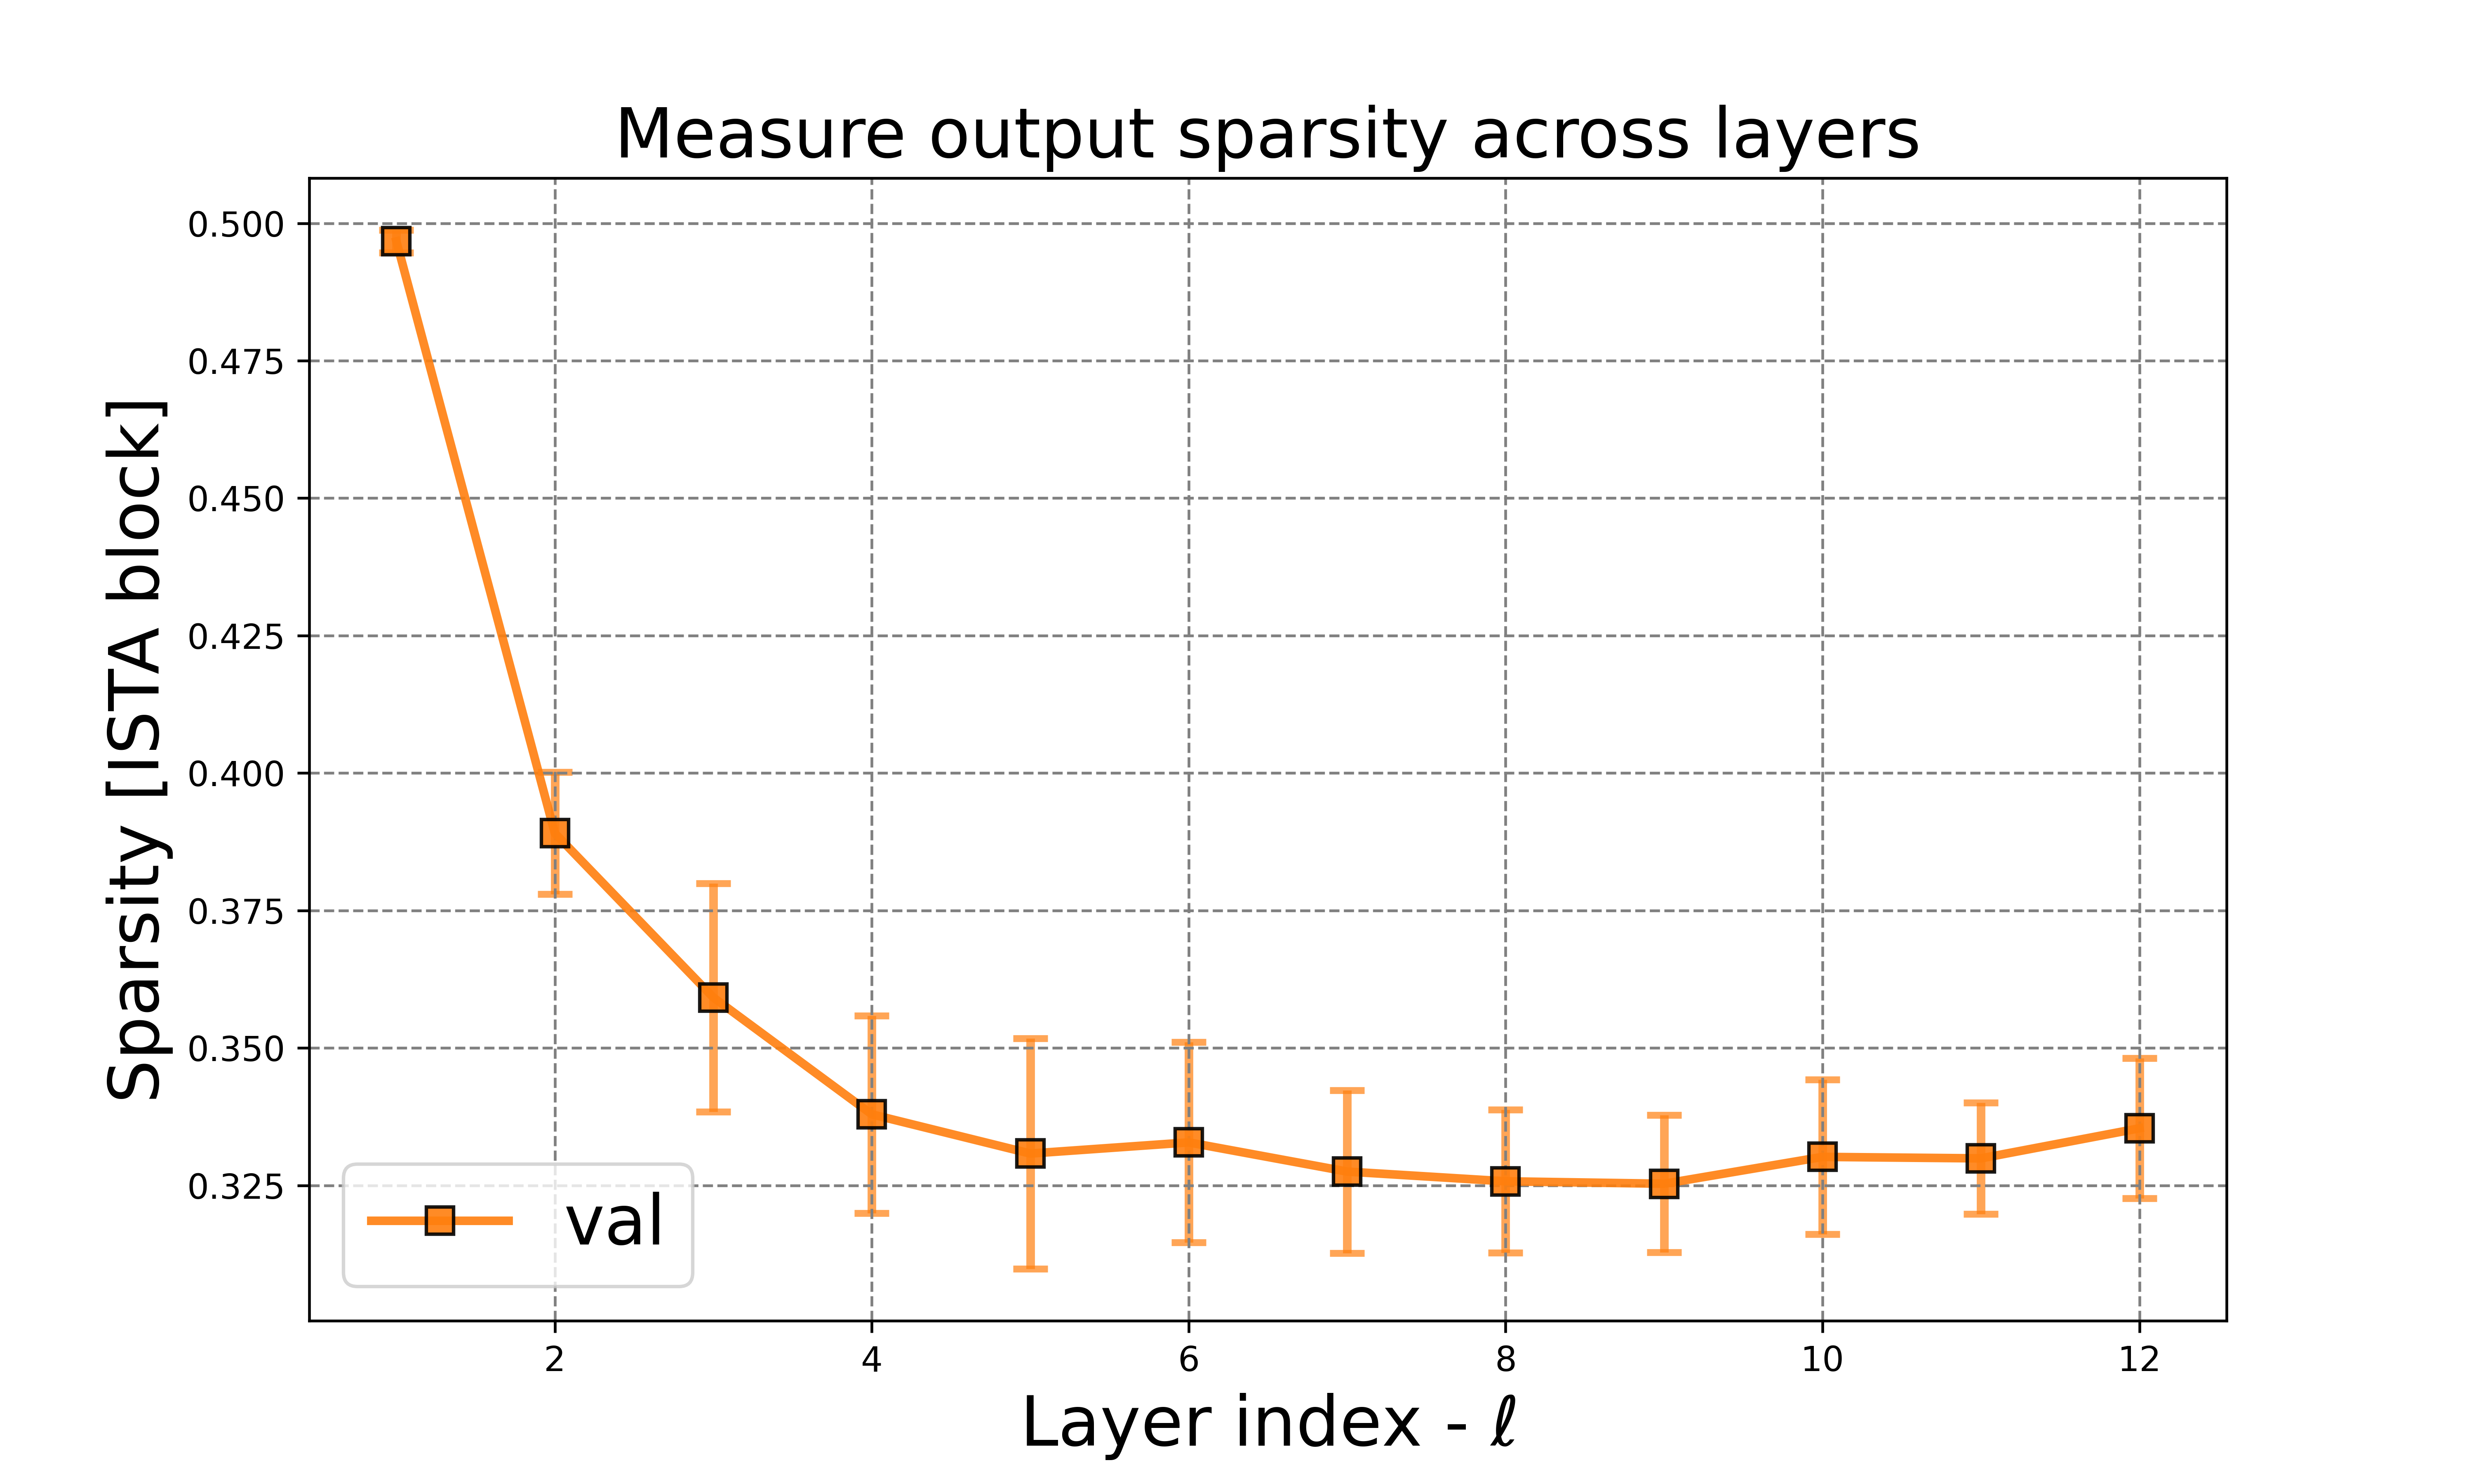
\includegraphics[width=\linewidth]{figs/original_sparsity.png}
\end{figure}


\begin{figure}[H]
	\caption{cr2 de mi red}
\centering
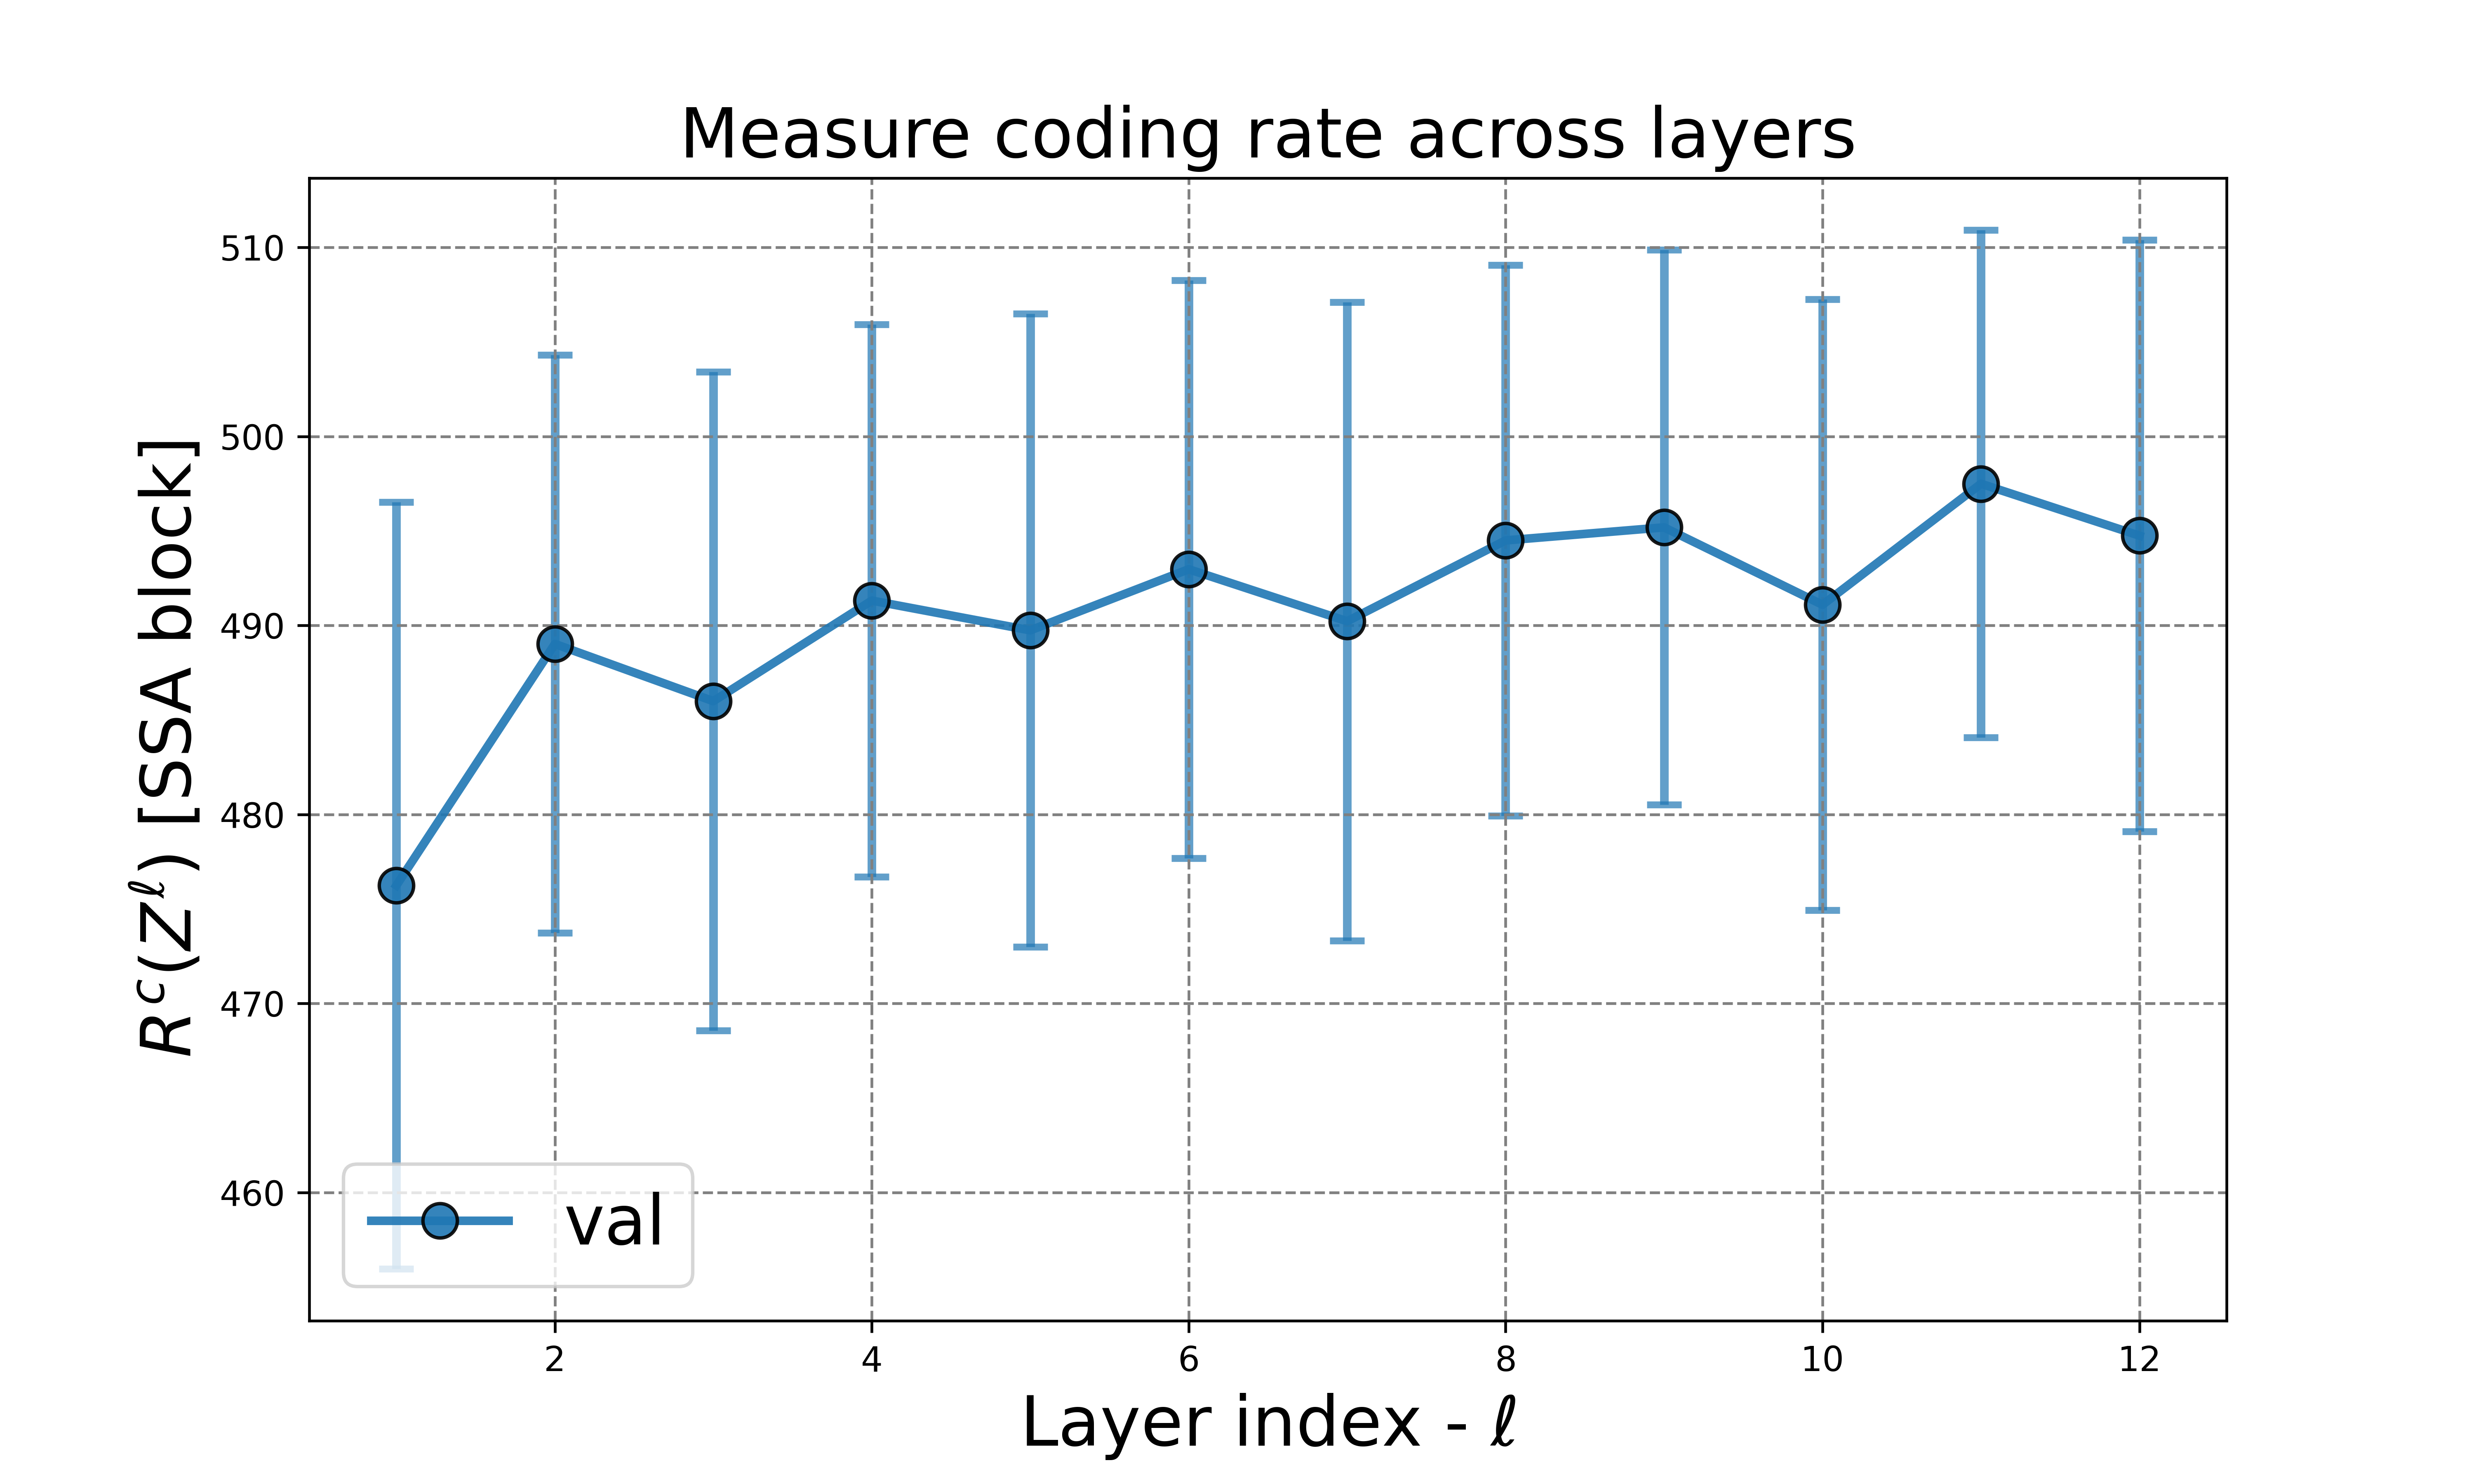
\includegraphics[width=\linewidth]{figs/mio_mcr2.png}
\end{figure}



\begin{figure}[H]
	\caption{cr2 de su red}
\centering
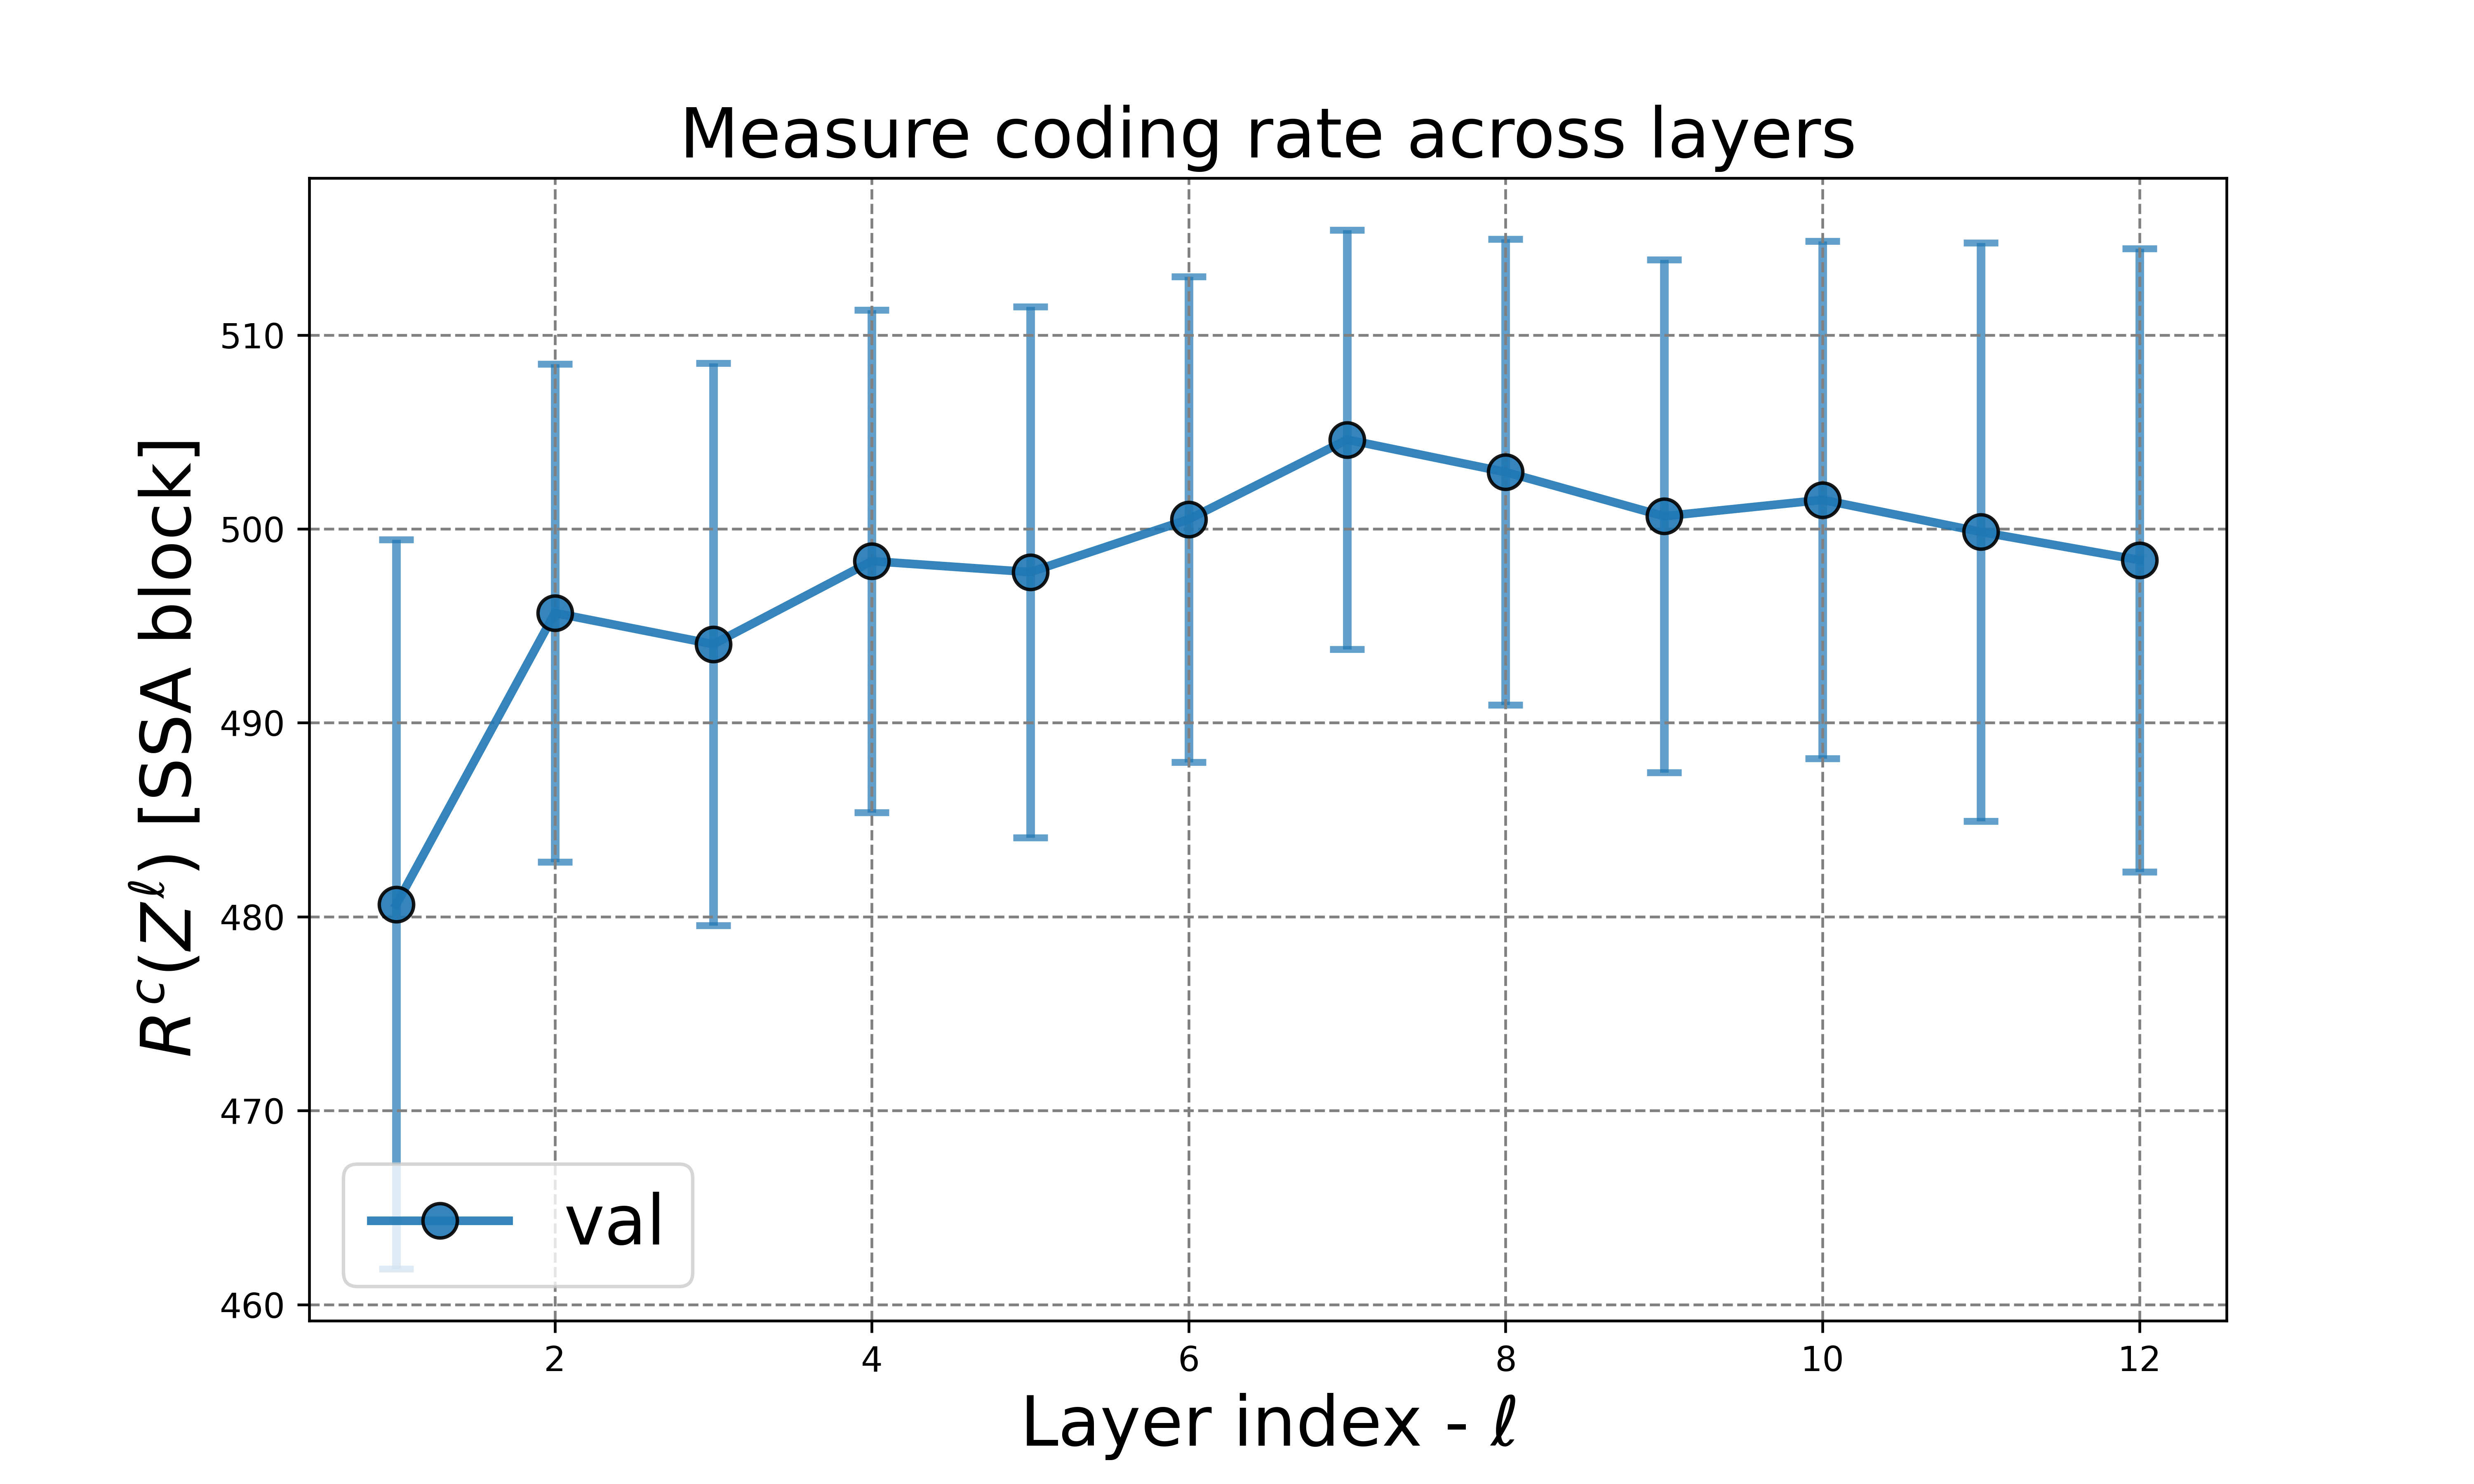
\includegraphics[width=\linewidth]{figs/original_mcr2.png}
\end{figure}














%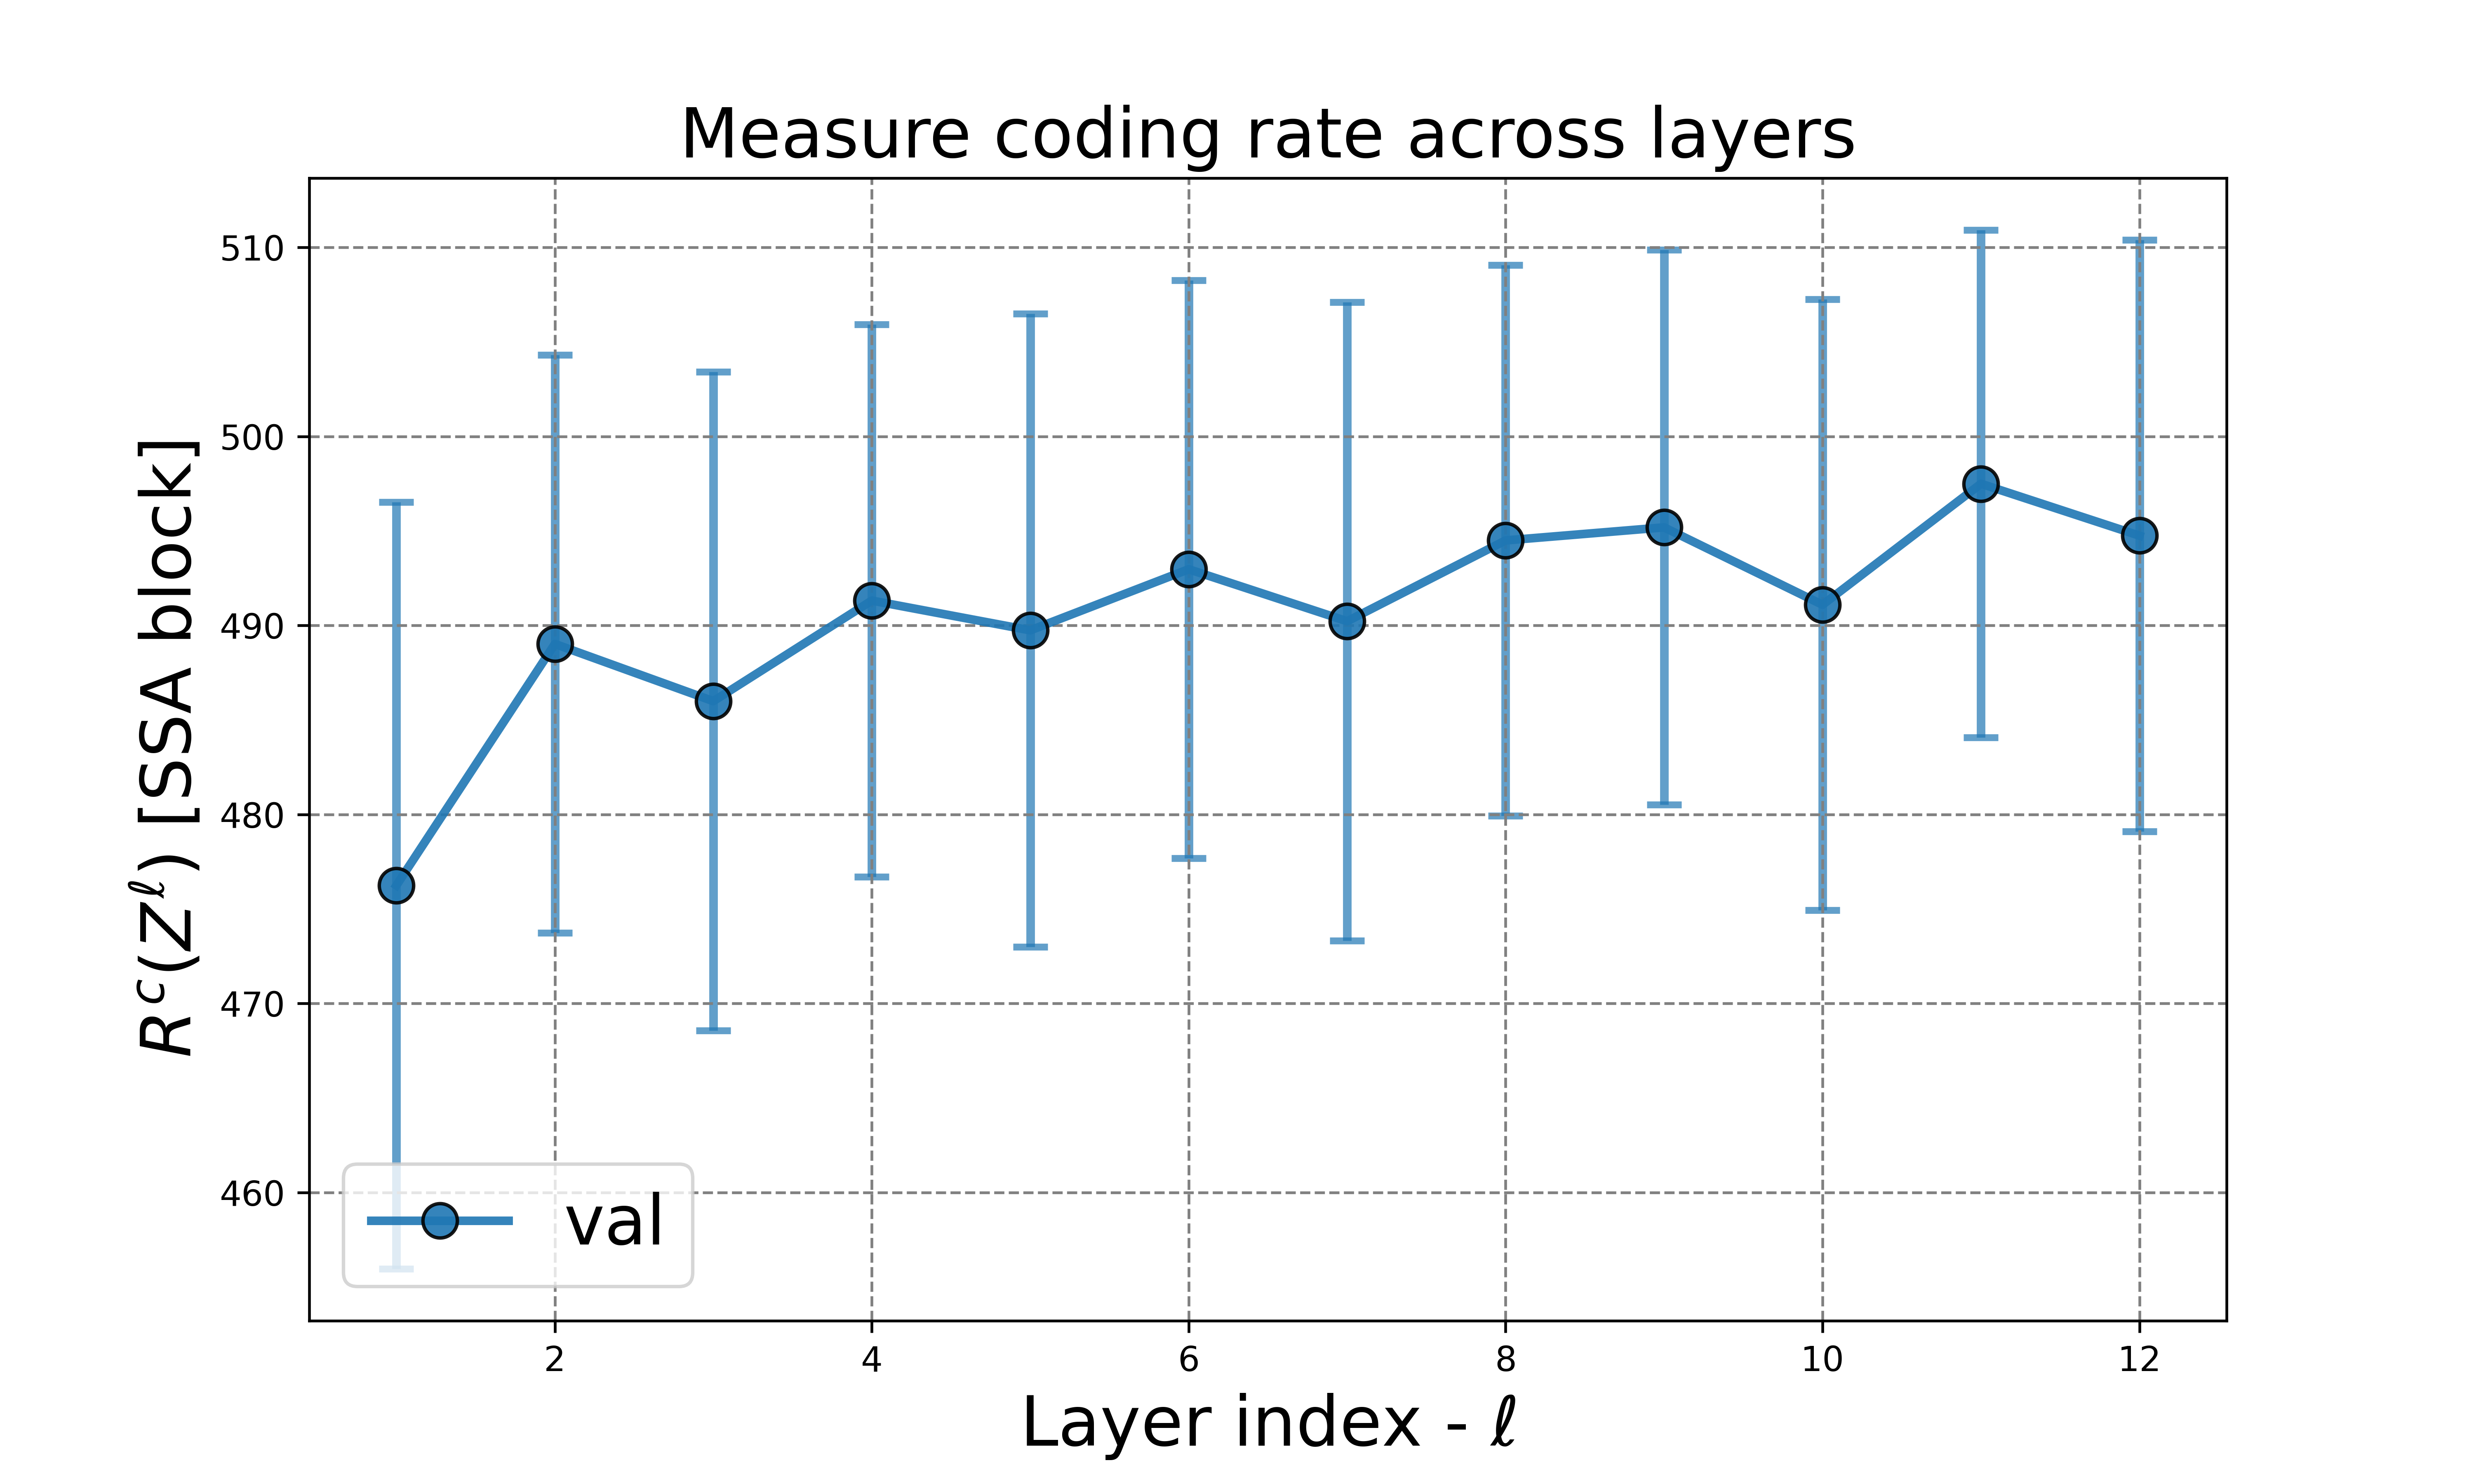
\includegraphics[width=\linewidth]{figs/mio_mcr2.png}
%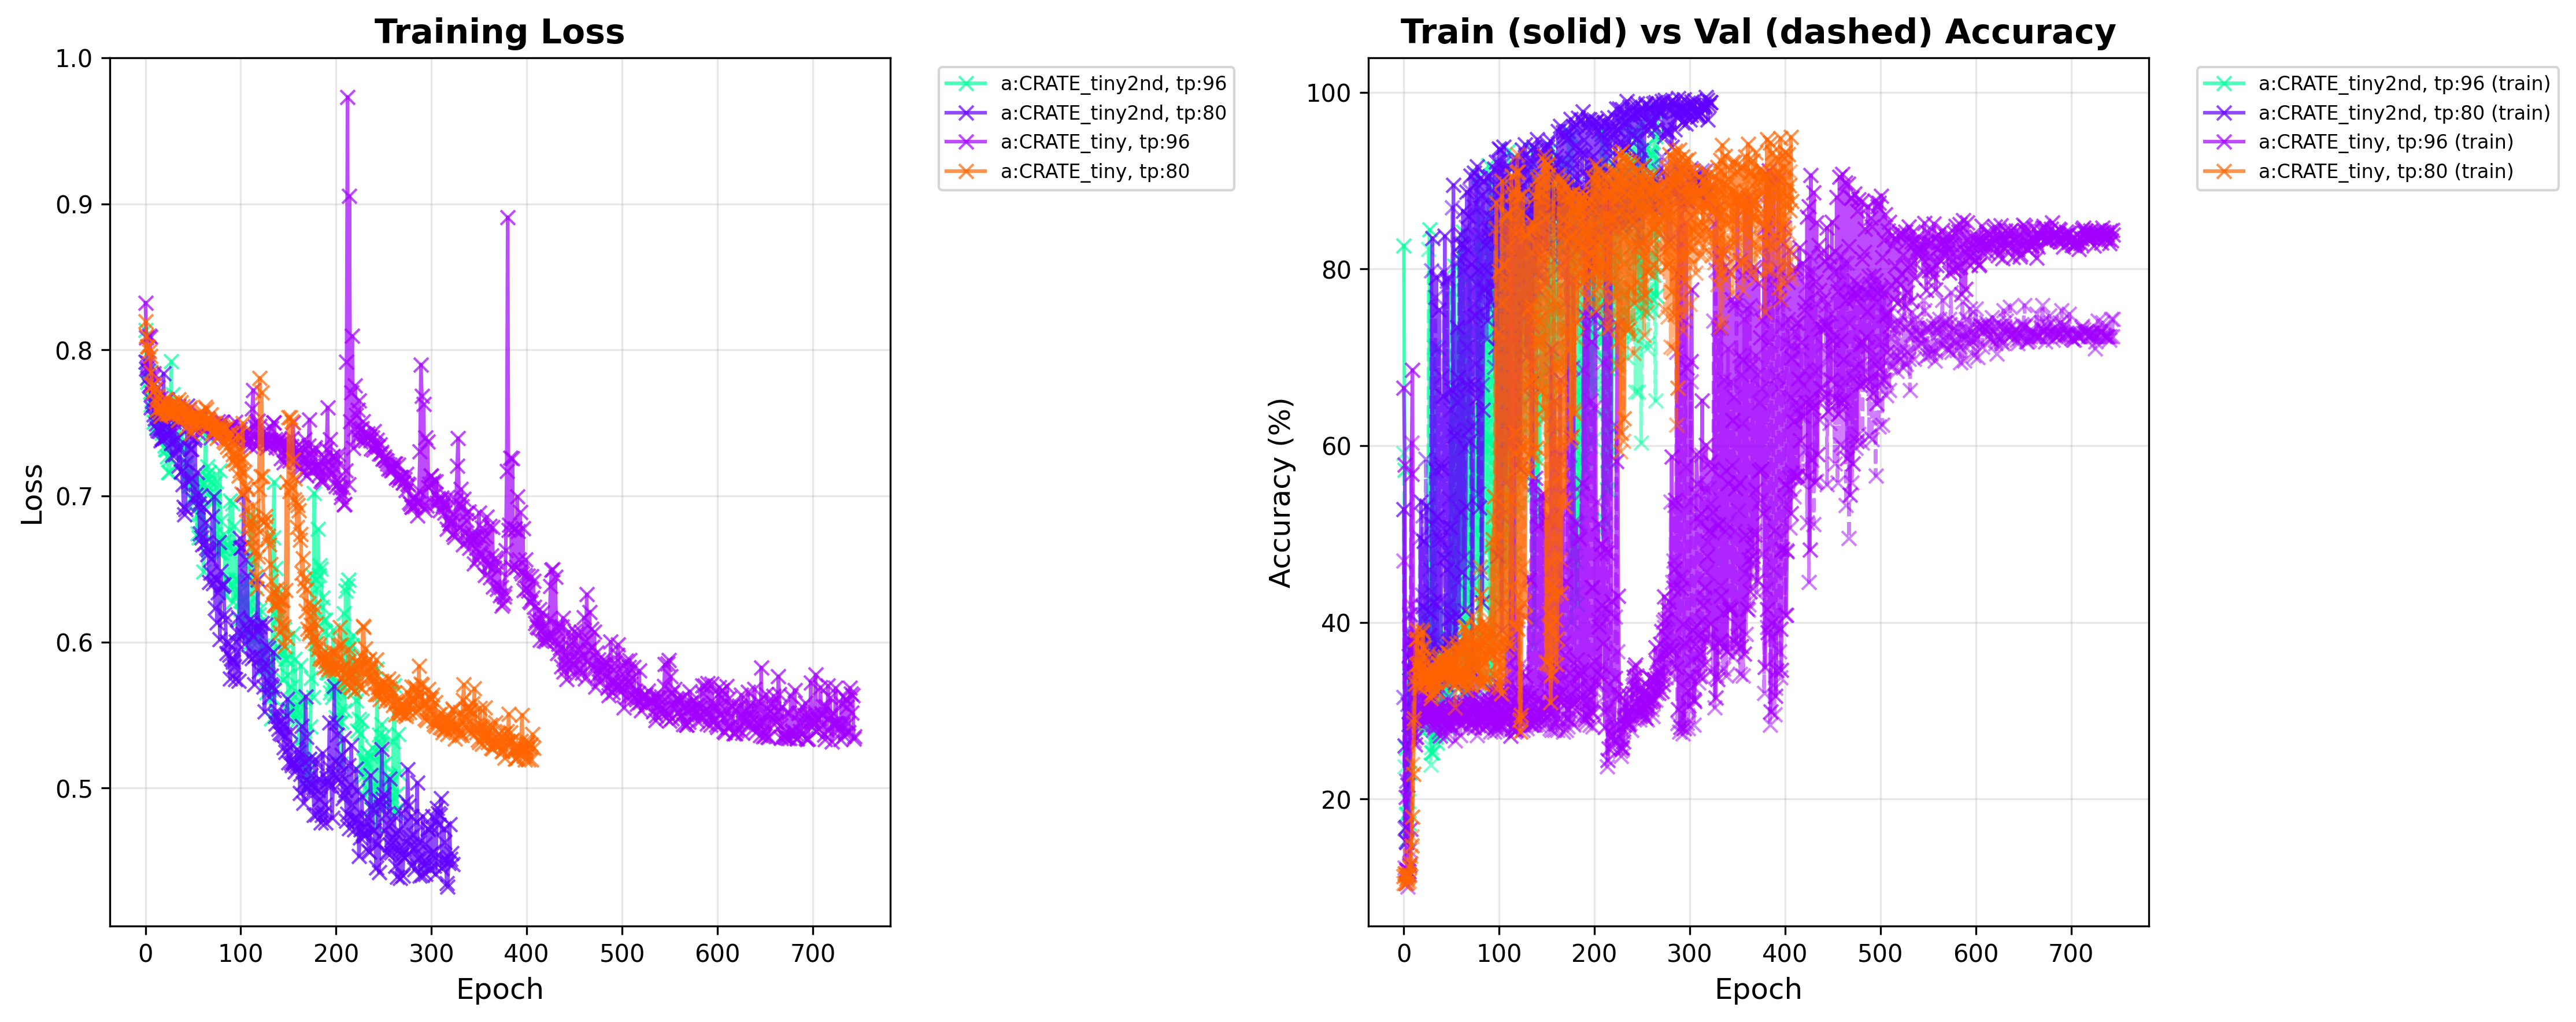
\includegraphics[width=\linewidth]{figs/9f3e62_e9f202_29b200_7bb28b_.png}
%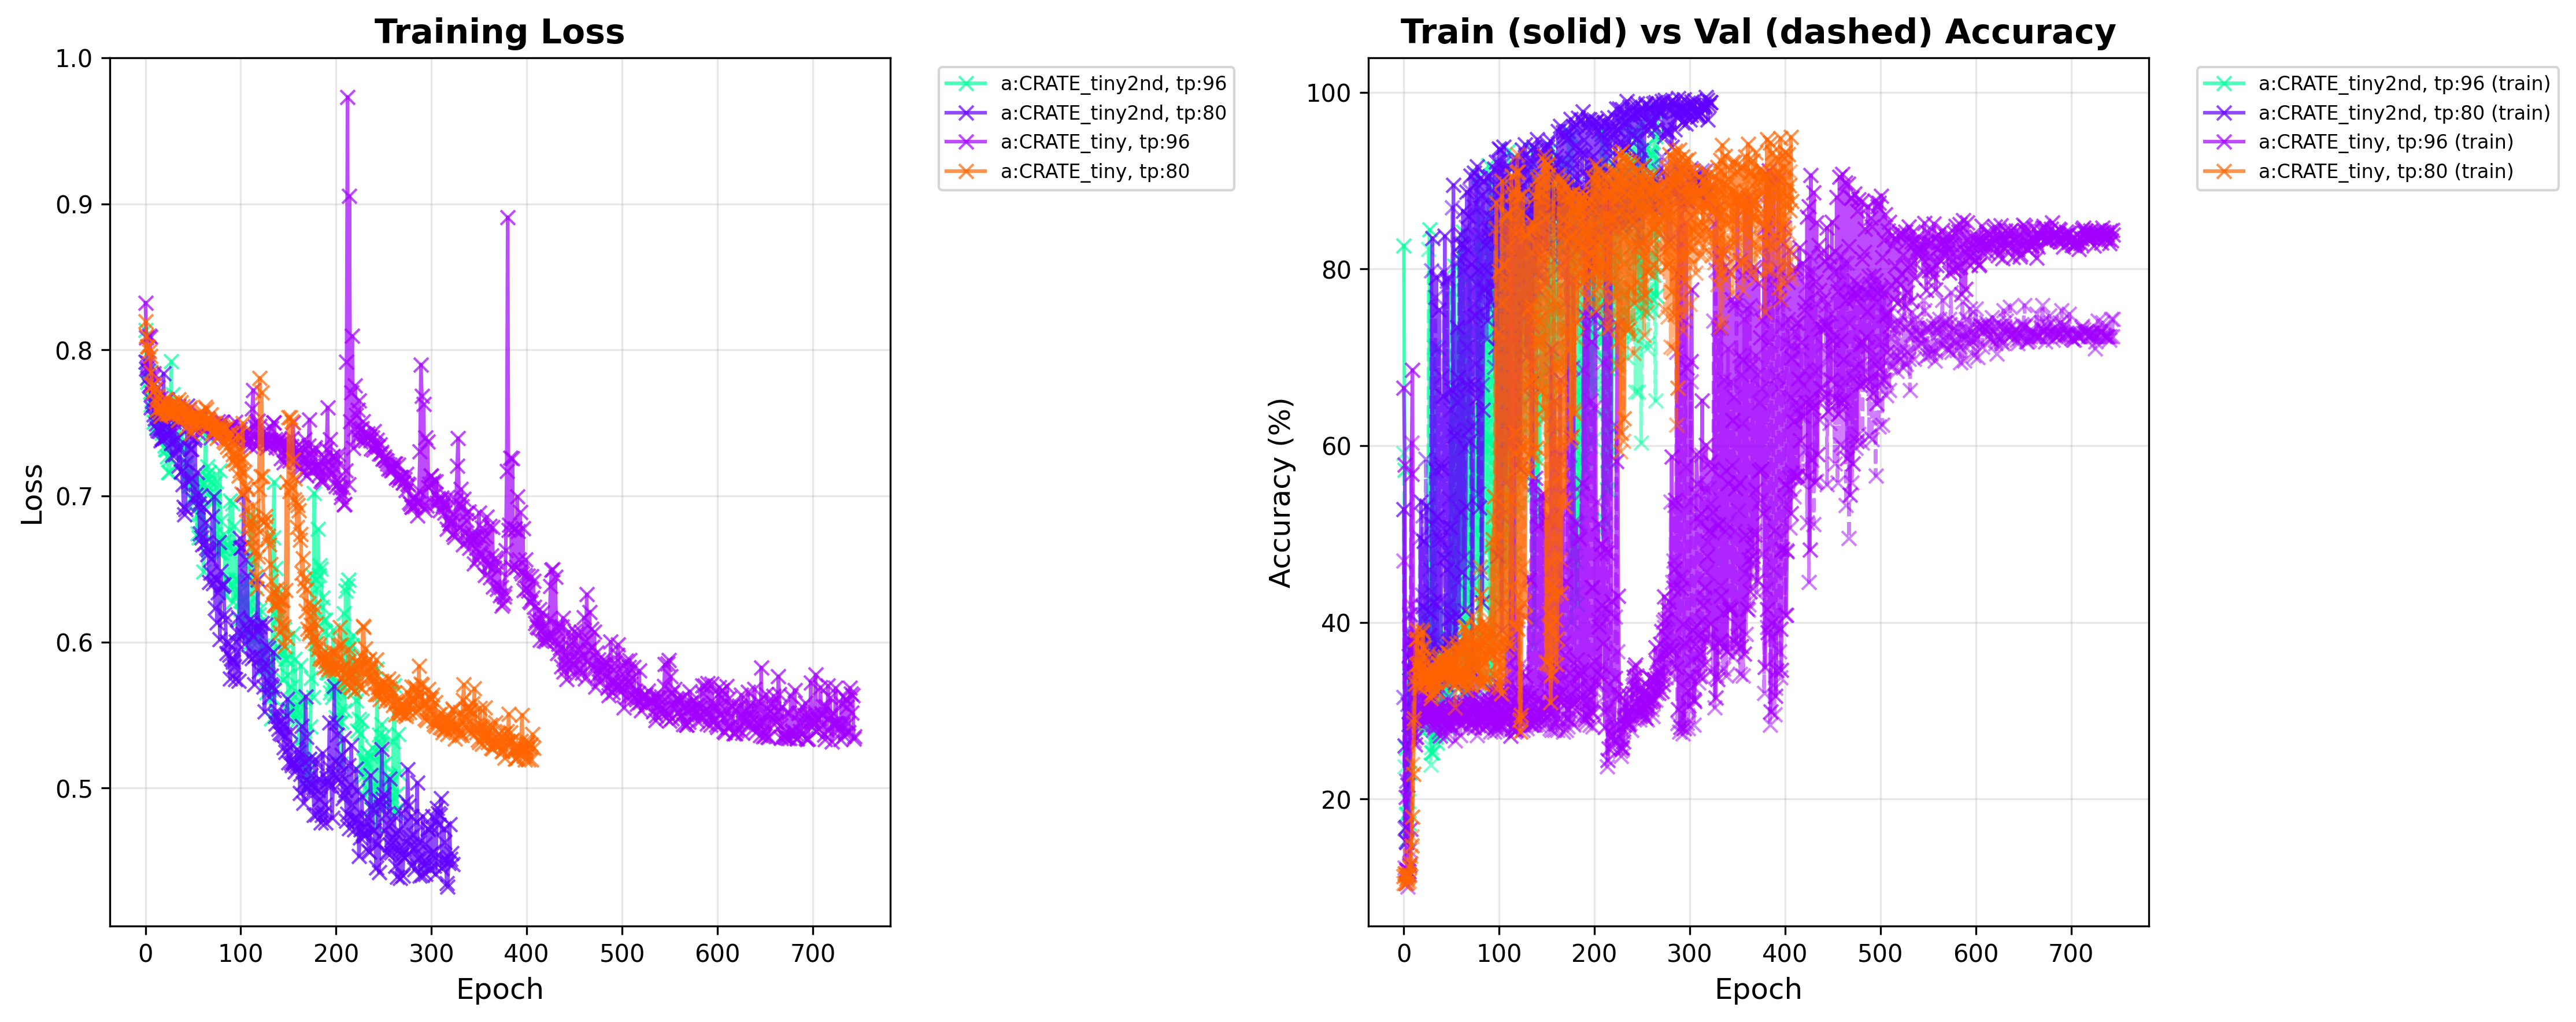
\includegraphics[width=\linewidth]{figs/9f3e62_e9f202_29b200_7bb28b_.png}
%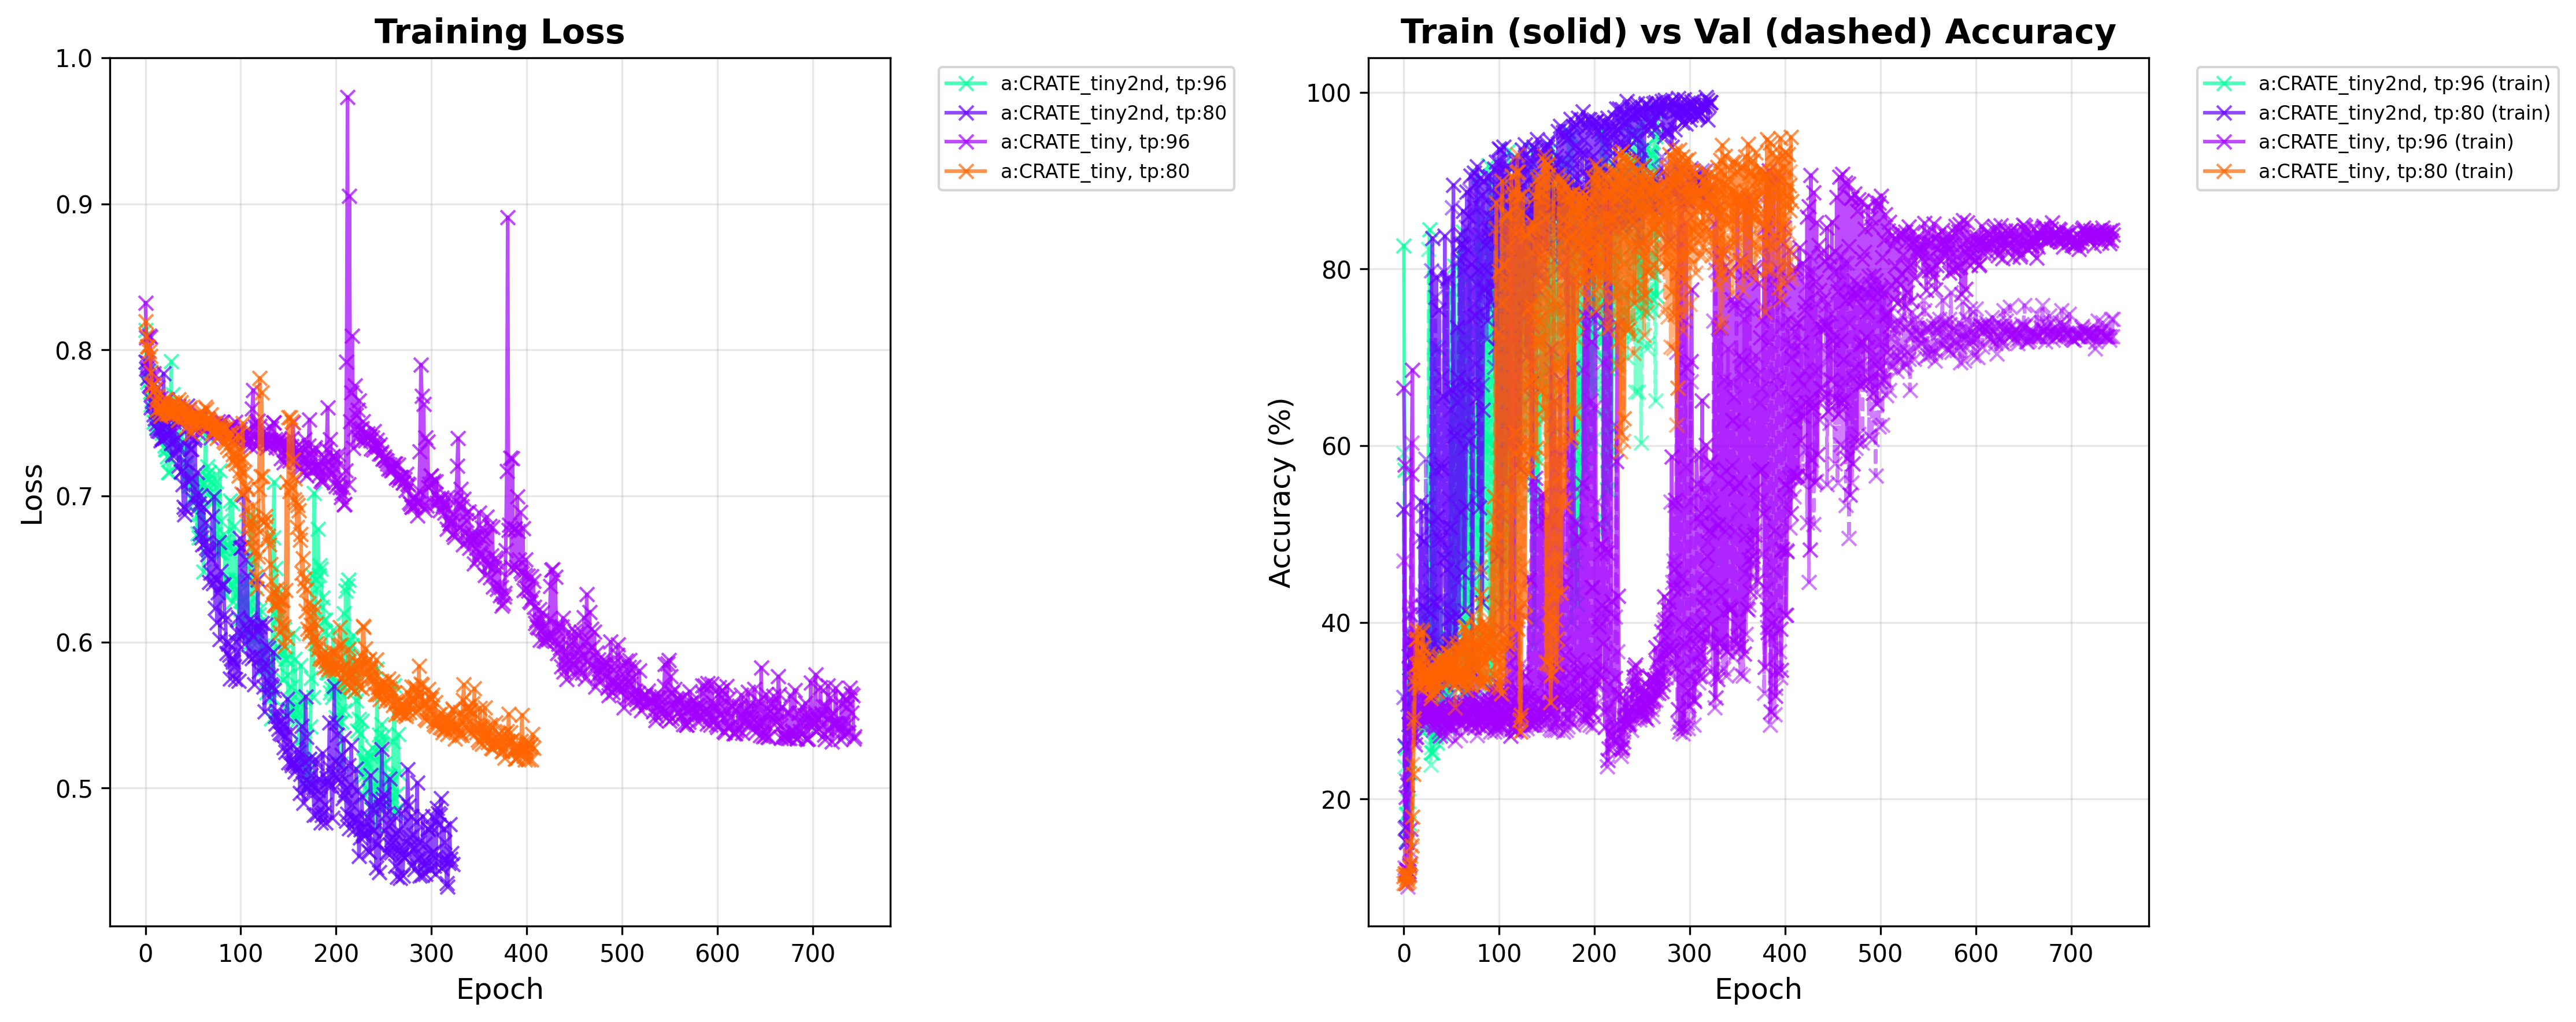
\includegraphics[width=\linewidth]{figs/9f3e62_e9f202_29b200_7bb28b_.png}
%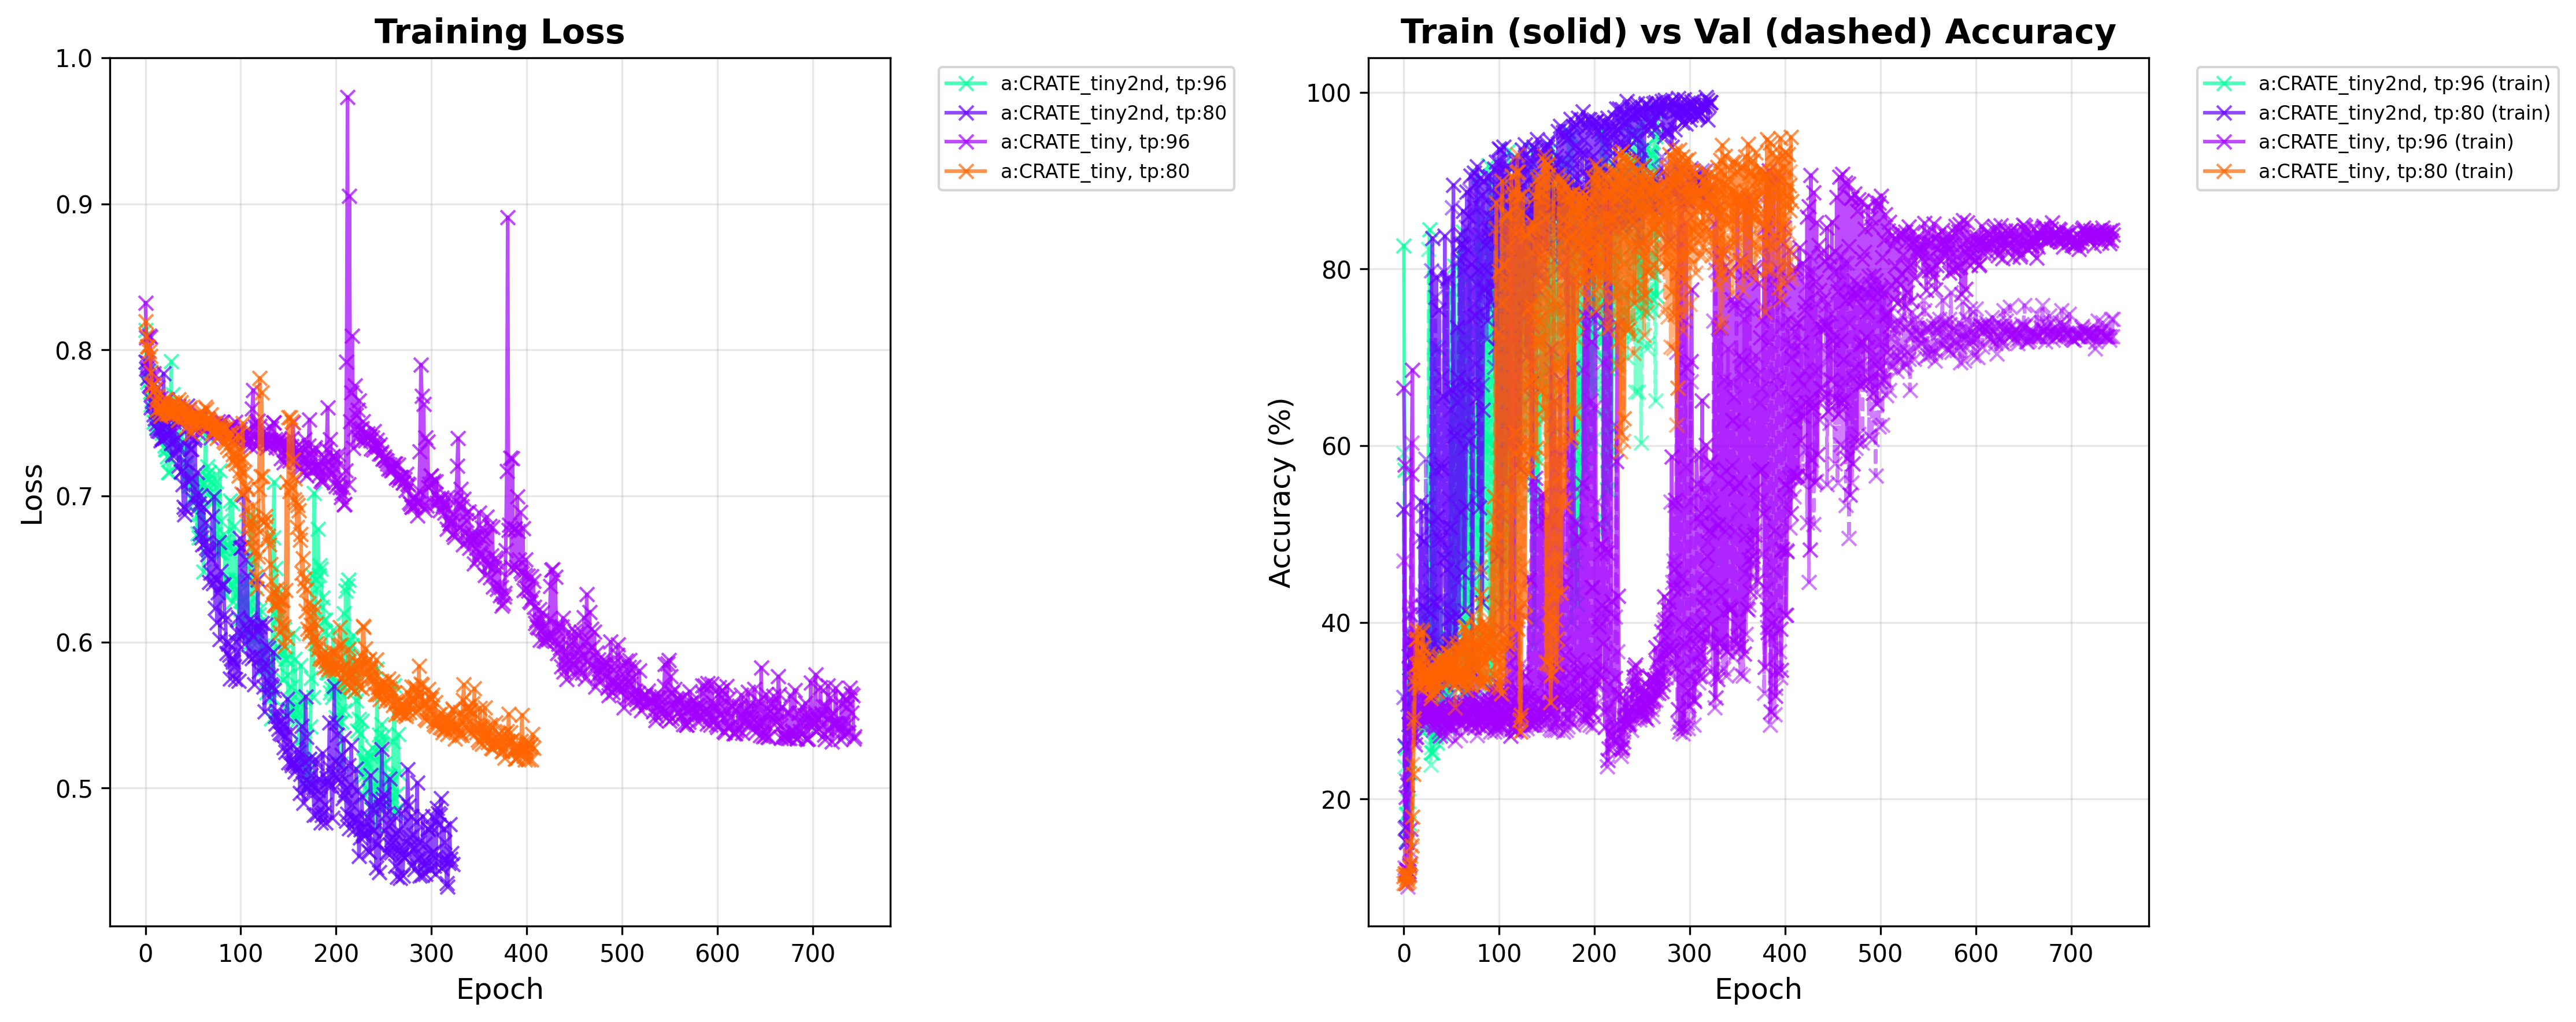
\includegraphics[width=\linewidth]{figs/9f3e62_e9f202_29b200_7bb28b_.png}
%
\includegraphics[width=\linewidth]{figs/enorme.png}
%\includegraphics[width=\linewidth]{figs/grande.png}
%\includegraphics[width=\linewidth]{figs/mediano.png}
%
\includegraphics[width=\linewidth]{figs/pequeño.png}
\end{document}
